\documentclass[11pt]{article}

\usepackage[utf8]{inputenc}
\usepackage{geometry}
\usepackage{graphicx}
\usepackage{amsmath}
\usepackage{amssymb}
\usepackage{booktabs}
\usepackage{hyperref}
\usepackage{float}

\geometry{a4paper, margin=1in}

\title{HW1 Report: From Scratch Three-Layer Neural Network for Fashion-MNIST}
\author{Yifan Luo \\ 23307130031}
\date{\today}

\begin{document}

\maketitle

\begin{abstract}
This work presents a from-scratch implementation of a three-layer multilayer perceptron (MLP) for image classification on the Fashion-MNIST dataset. The system includes manual implementations of forward and backward propagation, optimization with momentum, and learning rate scheduling. A structured hyperparameter search is conducted to identify effective configurations. The final model achieves a test accuracy of $90.53\%$. Experimental results highlight the role of dropout in mitigating overfitting and improving generalization.
\end{abstract}

\tableofcontents

\section{Introduction}

Modern deep learning frameworks abstract away many low-level details of model training, which can make it difficult to understand the underlying mechanisms. This work aims to bridge that gap by implementing a complete training pipeline for a three-layer MLP from scratch using NumPy.

The implementation covers all core components, including forward propagation, backpropagation, optimization, and data handling. The Fashion-MNIST dataset is used as a benchmark to evaluate the correctness and effectiveness of the system.

In addition, systematic hyperparameter tuning and experimental analysis are conducted to study training dynamics, generalization behavior, and learned feature representations.

\section{Dataset and Preprocessing}

\subsection{Fashion-MNIST Dataset}

The Fashion-MNIST dataset is a widely used benchmark for image classification tasks. It consists of grayscale images of fashion products, designed as a more challenging replacement for the MNIST handwritten digit dataset.

Each sample in the dataset is a $28 \times 28$ grayscale image, resulting in a 784-dimensional input after flattening. The dataset contains 10 classes, corresponding to different categories of clothing items:

\begin{itemize}
    \item T-shirt
    \item Trouser
    \item Pullover
    \item Dress
    \item Coat
    \item Sandal
    \item Shirt
    \item Sneaker
    \item Bag
    \item Ankle boot
\end{itemize}

The dataset is split into 60,000 training samples and 10,000 test samples. In this project, the original training set is further divided into a training set and a validation set for model selection.

To provide an intuitive understanding of the data distribution and visual characteristics, Figure~\ref{fig:data_visualization} shows the first ten samples along with their corresponding labels.

\begin{figure}[H]
    \centering
    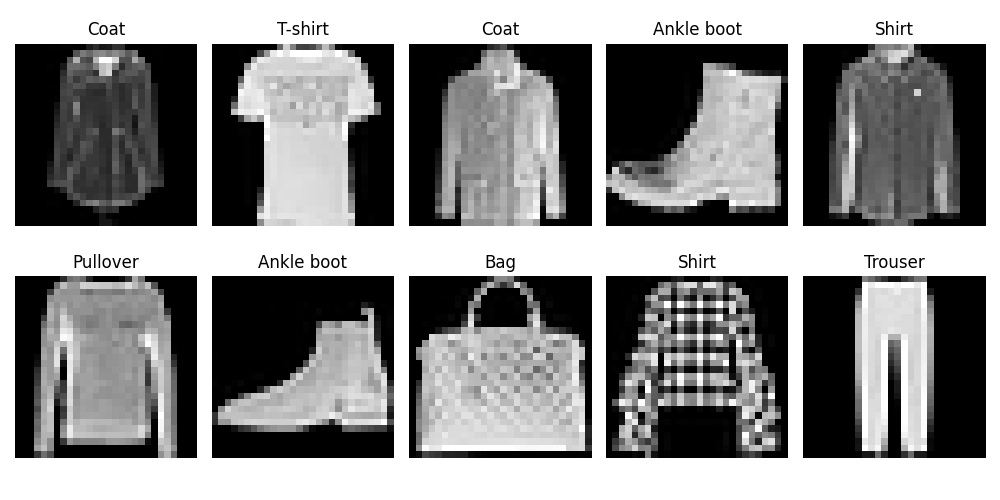
\includegraphics[width=0.8\linewidth]{../figures/data_visualization.png}
    \caption{Visualization of the first ten samples in the Fashion-MNIST dataset with their labels}
    \label{fig:data_visualization}
\end{figure}

\subsection{Data Splitting}

The original Fashion-MNIST training set (60,000 samples) is further divided into a training set and a validation set to support model selection and hyperparameter tuning. Specifically, a validation ratio of $0.1$ is used, resulting in $54{,}000$ training samples and $6{,}000$ validation samples.

This split is implemented via the \texttt{prepare\_data} function:
\begin{verbatim}
(X_train, y_train), (X_val, y_val), _ = prepare_data(..., val_ratio=0.1)
\end{verbatim}

The validation set is used exclusively for evaluating model performance during training and for selecting the best model checkpoint, while the training set is used for parameter optimization.

The test set (10,000 samples) remains untouched during training and validation, and is only used for final performance evaluation to ensure an unbiased estimate of generalization ability.

\subsection{Data Loading Pipeline}

A custom \texttt{DataLoader} is implemented to support mini-batch training. Given the input data $X \in \mathbb{R}^{N \times 784}$ and labels $y \in \mathbb{R}^{N}$, the pipeline performs the following operations:

\begin{itemize}
    \item \textbf{Normalization:} Pixel values are converted to \texttt{float32} and scaled to $[0, 1]$.
    \item \textbf{Mini-batch construction:} The dataset is divided into batches of size \texttt{batch\_size}.
    \item \textbf{Shuffling:} The training data is randomly shuffled at each epoch, while validation and test data remain in a fixed order.
\end{itemize}

During training, validation, and testing, separate data loaders are constructed:
\begin{verbatim}
train_loader = DataLoader(X_train, y_train, batch_size=..., shuffle=True)
val_loader   = DataLoader(X_val, y_val, batch_size=..., shuffle=False)
test_loader  = DataLoader(X_test, y_test, batch_size=..., shuffle=False)
\end{verbatim}

This design ensures efficient mini-batch processing and consistent evaluation across different stages of the pipeline.

\section{Model Architecture}

\subsection{Three-Layer MLP}

The model is a fully connected three-layer multilayer perceptron (MLP) for image classification. Given an input vector $x \in \mathbb{R}^{784}$, the network consists of two hidden layers followed by an output layer:

\[
\text{FC}_1 \rightarrow \text{Activation} \rightarrow \text{Dropout} \rightarrow
\text{FC}_2 \rightarrow \text{Activation} \rightarrow \text{Dropout} \rightarrow
\text{FC}_3
\]

where:
\begin{itemize}
    \item $\text{FC}_1: \mathbb{R}^{784} \rightarrow \mathbb{R}^{d_1}$
    \item $\text{FC}_2: \mathbb{R}^{d_1} \rightarrow \mathbb{R}^{d_2}$
    \item $\text{FC}_3: \mathbb{R}^{d_2} \rightarrow \mathbb{R}^{10}$
\end{itemize}

Here $d_1$ and $d_2$ denote the dimensions of the two hidden layers, which are treated as tunable hyperparameters.

The forward pass sequentially applies each layer, while the backward pass propagates gradients in the reverse order. Only the linear layers contain trainable parameters, which are optimized during training.

\subsection{Model Design Choices}

\paragraph{Activation Functions.}
The model supports multiple activation functions, including ReLU, Sigmoid, and Tanh. In practice, ReLU and Tanh are used in experiments. The same activation function is applied to both hidden layers.

\paragraph{Dropout.}
Dropout is applied after each activation layer to mitigate overfitting. During training, each activation is independently zeroed out with probability $p$. An inverted dropout scheme is adopted, where the remaining activations are scaled by $\frac{1}{1-p}$ to maintain the expected magnitude. During evaluation, dropout is disabled and the activations are passed through unchanged.

\paragraph{Weight Initialization.}
The initialization method is automatically selected based on the activation function. He initialization is used for ReLU, while Xavier initialization is used for Sigmoid and Tanh, ensuring stable variance of activations across layers.

\section{Loss Function and Regularization}

\subsection{Cross-Entropy Loss}

For multi-class classification, the cross-entropy loss is used. Given the logits $Z \in \mathbb{R}^{N \times C}$ and ground-truth labels $y \in \{0, \dots, C-1\}^N$, the predicted probabilities are obtained via the softmax function.

For numerical stability, the logits are shifted before exponentiation:
\[
\tilde{Z}_{i,j} = Z_{i,j} - \max_{k} Z_{i,k}
\]

The softmax probabilities are then computed as:
\[
P_{i,j} = \frac{\exp(\tilde{Z}_{i,j})}{\sum_{k=1}^{C} \exp(\tilde{Z}_{i,k})}
\]

The loss is defined as the average negative log-likelihood:
\[
L = -\frac{1}{N} \sum_{i=1}^{N} \log P_{i, y_i}
\]

\subsection{L2 Regularization}

To reduce overfitting, L2 regularization (weight decay) is applied to all linear layers. The regularization term is defined as:
\[
L_{\text{reg}} = \frac{\lambda}{2} \sum_{l} \| W^{(l)} \|_F^2
\]
where $\lambda$ is the weight decay coefficient and $W^{(l)}$ denotes the weight matrix of the $l$-th layer.

The total loss is given by:
\[
L_{\text{total}} = L + L_{\text{reg}}
\]

\section{From-Scratch Backpropagation System}

\subsection{Design Overview}

The backpropagation system is implemented in a modular manner. Each layer explicitly defines its own \texttt{forward} and \texttt{backward} functions, and is responsible for computing local gradients.

During the forward pass, intermediate variables required for gradient computation are cached within each layer. In the backward pass, gradients are propagated in reverse order through the network by sequentially invoking each layer's \texttt{backward} method.

At the model level, backpropagation is implemented as:
\begin{verbatim}
for layer in reversed(self.layers):
    dout = layer.backward(dout)
\end{verbatim}

This design follows the chain rule and allows gradients to flow through the entire network in a structured manner.

\subsection{Layer-wise Gradient Computation}

\paragraph{Loss Layer.}
For the softmax cross-entropy loss, the gradient with respect to the logits is:
\[
\frac{\partial L}{\partial Z} = \frac{1}{N} (P - Y)
\]
where $P$ is the predicted probability matrix and $Y$ is the one-hot encoding of the labels.

\paragraph{Linear Layer.}
For a linear transformation $Z = XW + b$, the gradients are computed as:
\[
\frac{\partial L}{\partial W} = X^\top \frac{\partial L}{\partial Z} + \lambda W, \quad
\frac{\partial L}{\partial b} = \mathbf{1}^\top \frac{\partial L}{\partial Z}, \quad
\frac{\partial L}{\partial X} = \frac{\partial L}{\partial Z} W^\top
\]
where $\mathbf{1}$ is an all-ones vector and $\lambda$ is the weight decay coefficient.

\paragraph{Activation Functions.}
Activation layers apply element-wise nonlinearities and compute gradients using their local derivatives:
\begin{itemize}
    \item ReLU: $\frac{\partial L}{\partial Z} = \frac{\partial L}{\partial A} \cdot \mathbf{I}(Z > 0)$
    \item Sigmoid: $\frac{\partial L}{\partial Z} = \frac{\partial L}{\partial A} \cdot A(1 - A)$
    \item Tanh: $\frac{\partial L}{\partial Z} = \frac{\partial L}{\partial A} \cdot (1 - A^2)$
\end{itemize}

\paragraph{Dropout Layer.}
During training, dropout applies a binary mask to the activations. In the backward pass, the same mask is applied to the gradients. When dropout is inactive, gradients pass through unchanged.

\subsection{Gradient Control Mechanism}

A global gradient control mechanism is implemented to support inference without storing intermediate states. Specifically, a context manager (\texttt{no\_grad}) disables caching during the forward pass.

When gradient tracking is disabled, layers do not store intermediate variables, and the backward pass cannot be invoked. This reduces memory usage during evaluation.

\section{Optimization Strategy}

\subsection{SGD with Momentum}

Model parameters are optimized using stochastic gradient descent (SGD) with momentum. For each parameter $\theta$, the update rule is:
\[
v_t = \mu v_{t-1} + g_t, \quad
\theta_t = \theta_{t-1} - \eta v_t
\]
where $g_t = \nabla_{\theta} L$ is the gradient at step $t$, $\eta$ is the learning rate, and $\mu$ is the momentum coefficient.

Momentum accumulates a running average of past gradients, which helps accelerate convergence along consistent descent directions and reduces oscillations in high-curvature regions.

\subsection{Learning Rate Scheduling}

A learning rate scheduler is used to adjust the step size during training. Several scheduling strategies are implemented, including constant, step decay, linear decay, and cosine annealing.

In the experiments, cosine annealing is used. The learning rate at step $t$ is given by:
\[
\eta_t = \frac{1}{2} \eta_0 \left(1 + \cos\left(\frac{\pi t}{T}\right)\right)
\]
where $\eta_0$ is the initial learning rate and $T$ is the total number of steps.

This schedule smoothly decreases the learning rate from $\eta_0$ to $0$, enabling large updates in early stages and more refined updates as training progresses.

\section{Training Pipeline}

\subsection{Training Loop}

Training is performed in a mini-batch manner over multiple epochs. For each batch, the following steps are executed:

\begin{itemize}
    \item \textbf{Forward pass:} Compute logits and the data loss using the cross-entropy criterion.
    \item \textbf{Loss aggregation:} Add the L2 regularization term to obtain the total loss.
    \item \textbf{Backward pass:} Compute gradients with respect to all model parameters.
    \item \textbf{Parameter update:} Update parameters using SGD with momentum.
\end{itemize}

The learning rate is updated by a scheduler during training. For iteration-based schedules (e.g., cosine and linear decay), the update is performed at each iteration. For epoch-based schedules (e.g., step decay), the learning rate is updated periodically based on the predefined schedule.

Training statistics, including loss and learning rate, are recorded at both iteration and epoch levels for later analysis.

\subsection{Validation and Model Selection}

At the end of each epoch, the model is evaluated on the validation set. The validation accuracy is used as the primary metric for model selection.

The model achieving the highest validation accuracy is saved as the best checkpoint. Along with the model weights, a metadata file is stored to record the training state and key hyperparameters.

This strategy selects the model with the best observed validation performance, which serves as a proxy for generalization.

\subsection{Resume Training}

The training pipeline supports resuming from a saved checkpoint by restoring model weights and basic training state, allowing training to continue from a previous point.

\section{Hyperparameter Search}

\subsection{Search Strategy}

Hyperparameter tuning is conducted using grid search. Although both grid search and random search are implemented, all experiments in this work adopt grid search for its exhaustive coverage of the search space.

To balance computational cost and search quality, the number of training epochs during search is reduced (30 epochs), and a fixed training configuration is used, including momentum ($0.9$) and cosine learning rate scheduling.

The search process is organized in two stages.

\subsection{Stage I: Baseline Search without Dropout}

In the first stage, hyperparameters are tuned without dropout to establish a baseline configuration. The search space includes learning rate, hidden layer dimensions, weight decay, activation function, and batch size.

Figure~\ref{fig:search1_corr} shows the correlation between each hyperparameter and validation accuracy. The learning rate exhibits the strongest correlation (0.91), indicating that $10^{-2}$ consistently outperforms $10^{-3}$. Batch size also shows a noticeable effect, where smaller batches ($32$) achieve better performance. In addition, a mild positive correlation is observed for the first hidden layer size, suggesting that a larger dimension ($512$) is slightly more favorable on average. Other hyperparameters have weaker marginal effects.

\begin{figure}[H]
    \centering
    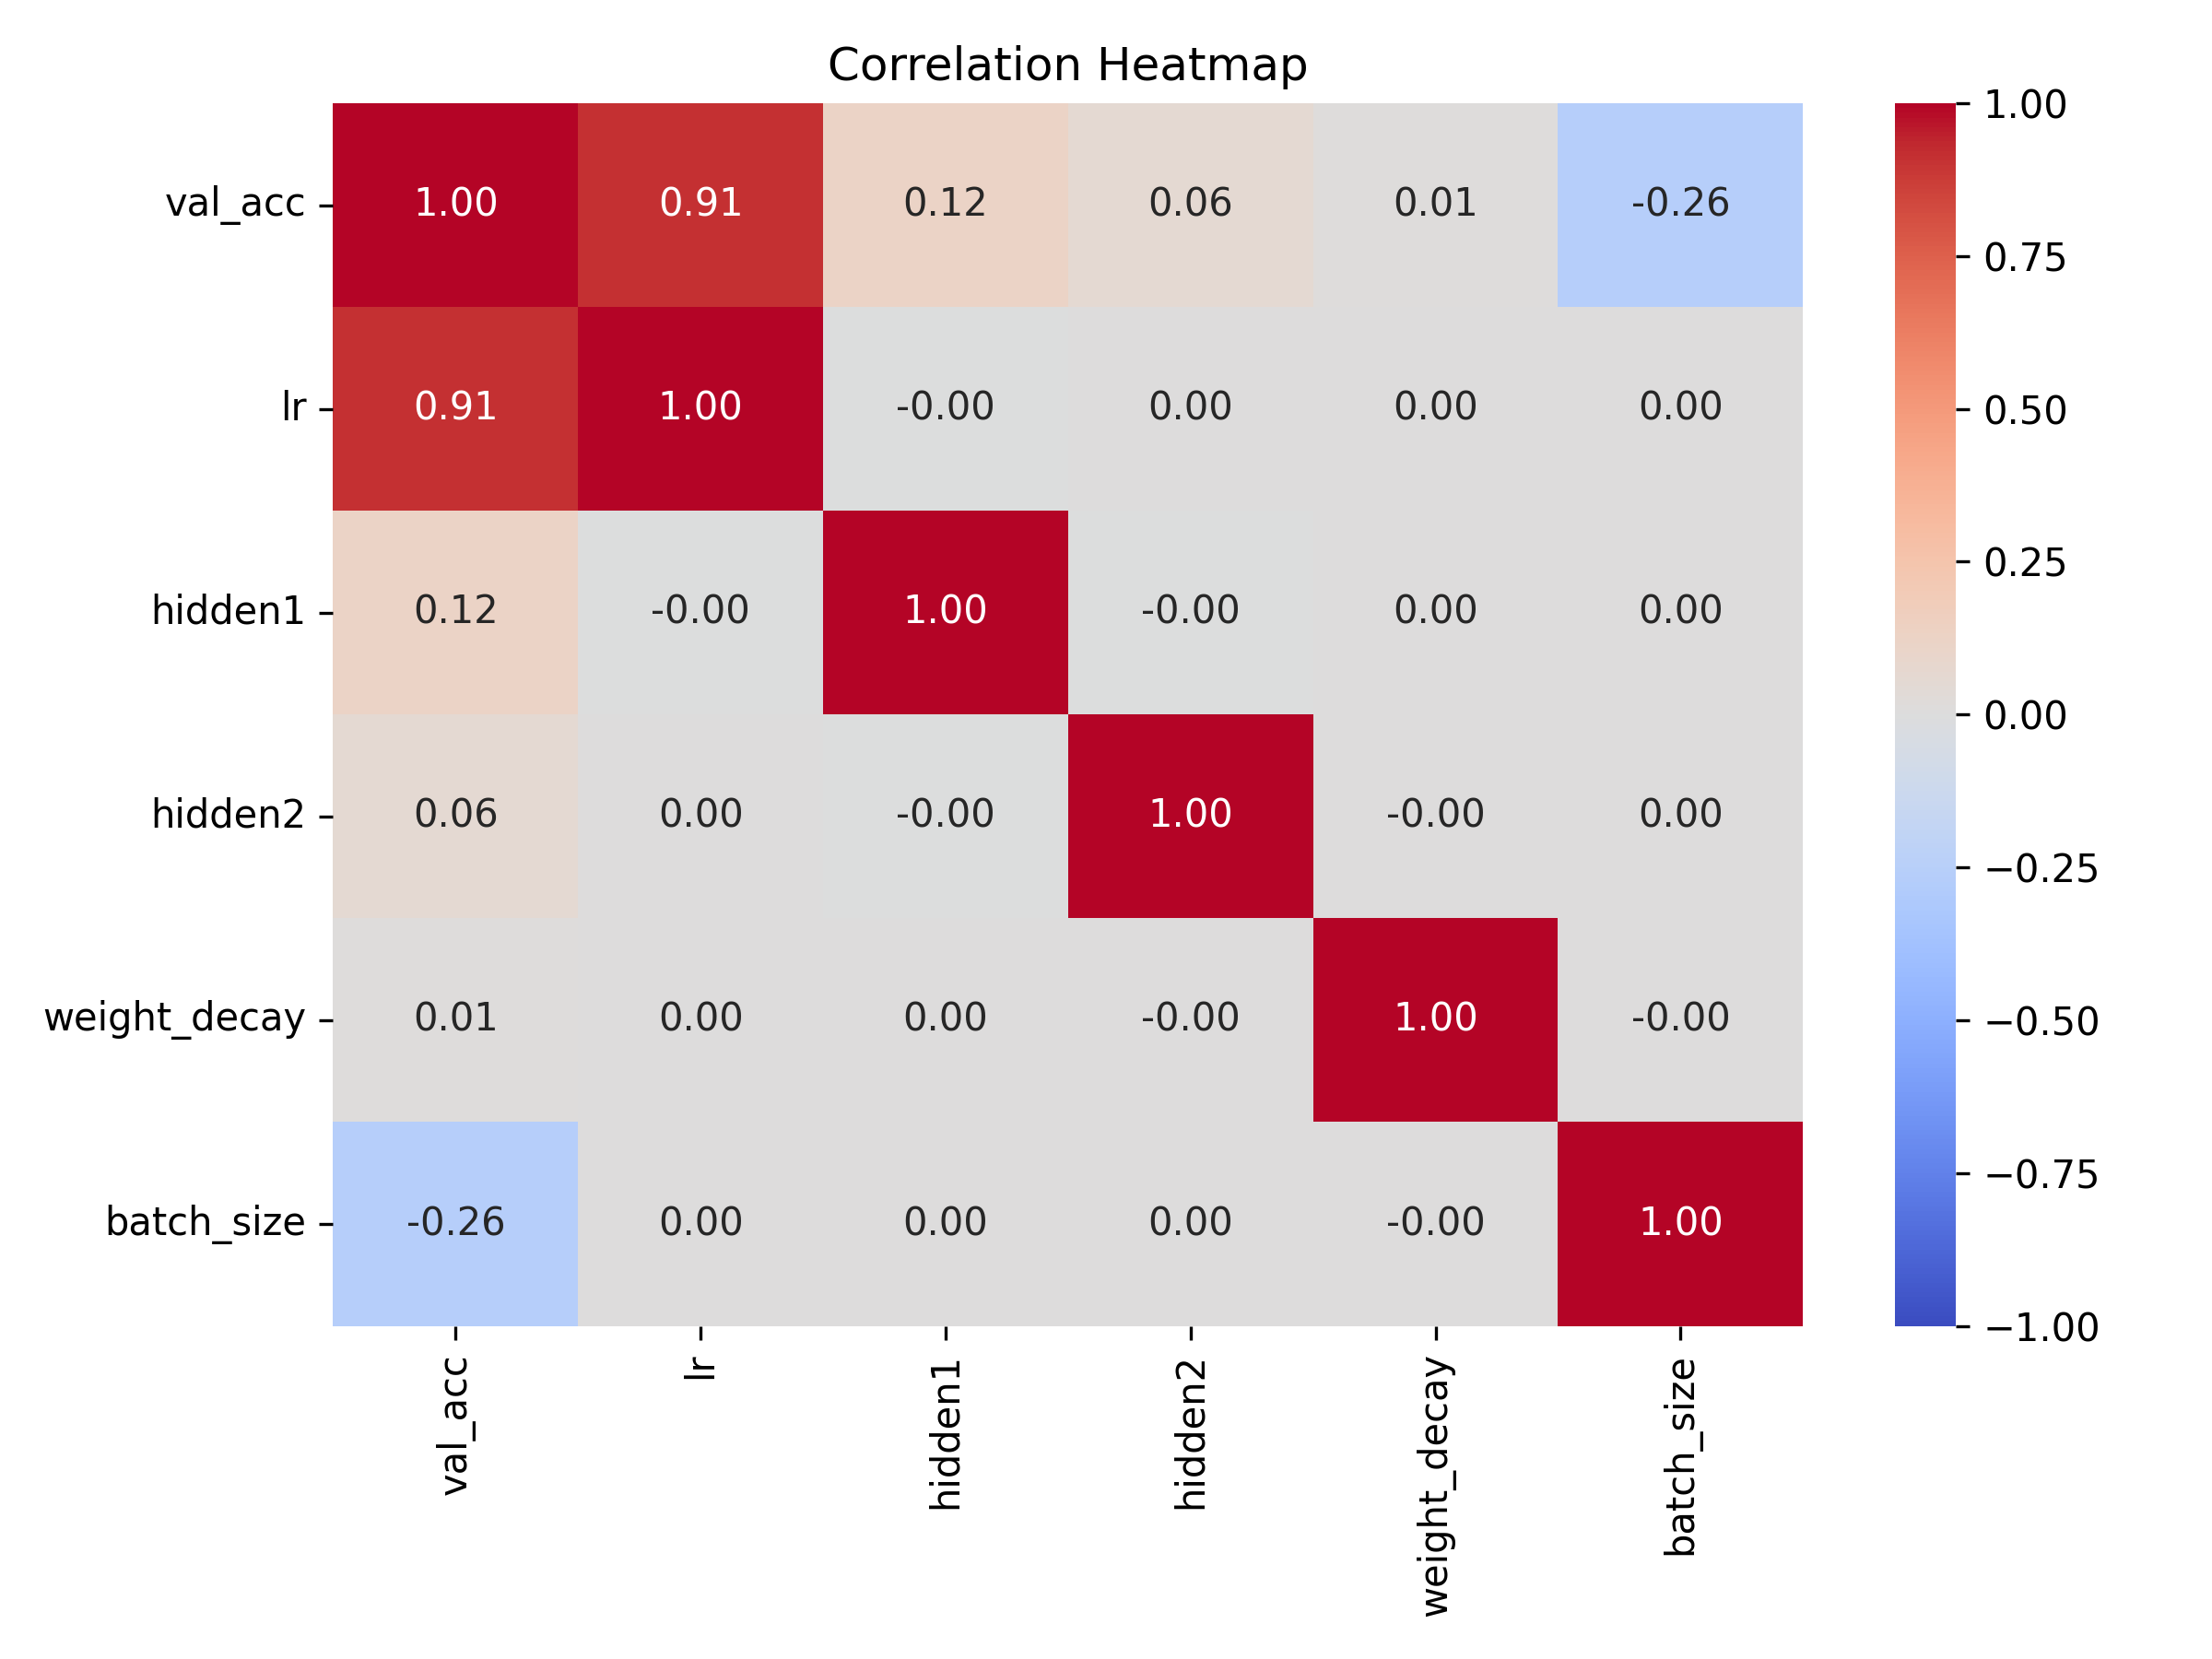
\includegraphics[width=0.7\linewidth]{../figures/search_1_correlation_heatmap.png}
    \caption{Correlation between hyperparameters and validation accuracy (Stage I)}
    \label{fig:search1_corr}
\end{figure}

The marginal effects are further illustrated in Figure~\ref{fig:search1_marginal}, where learning rate, batch size, and activation function show consistent trends.

\begin{figure}[H]
    \centering
    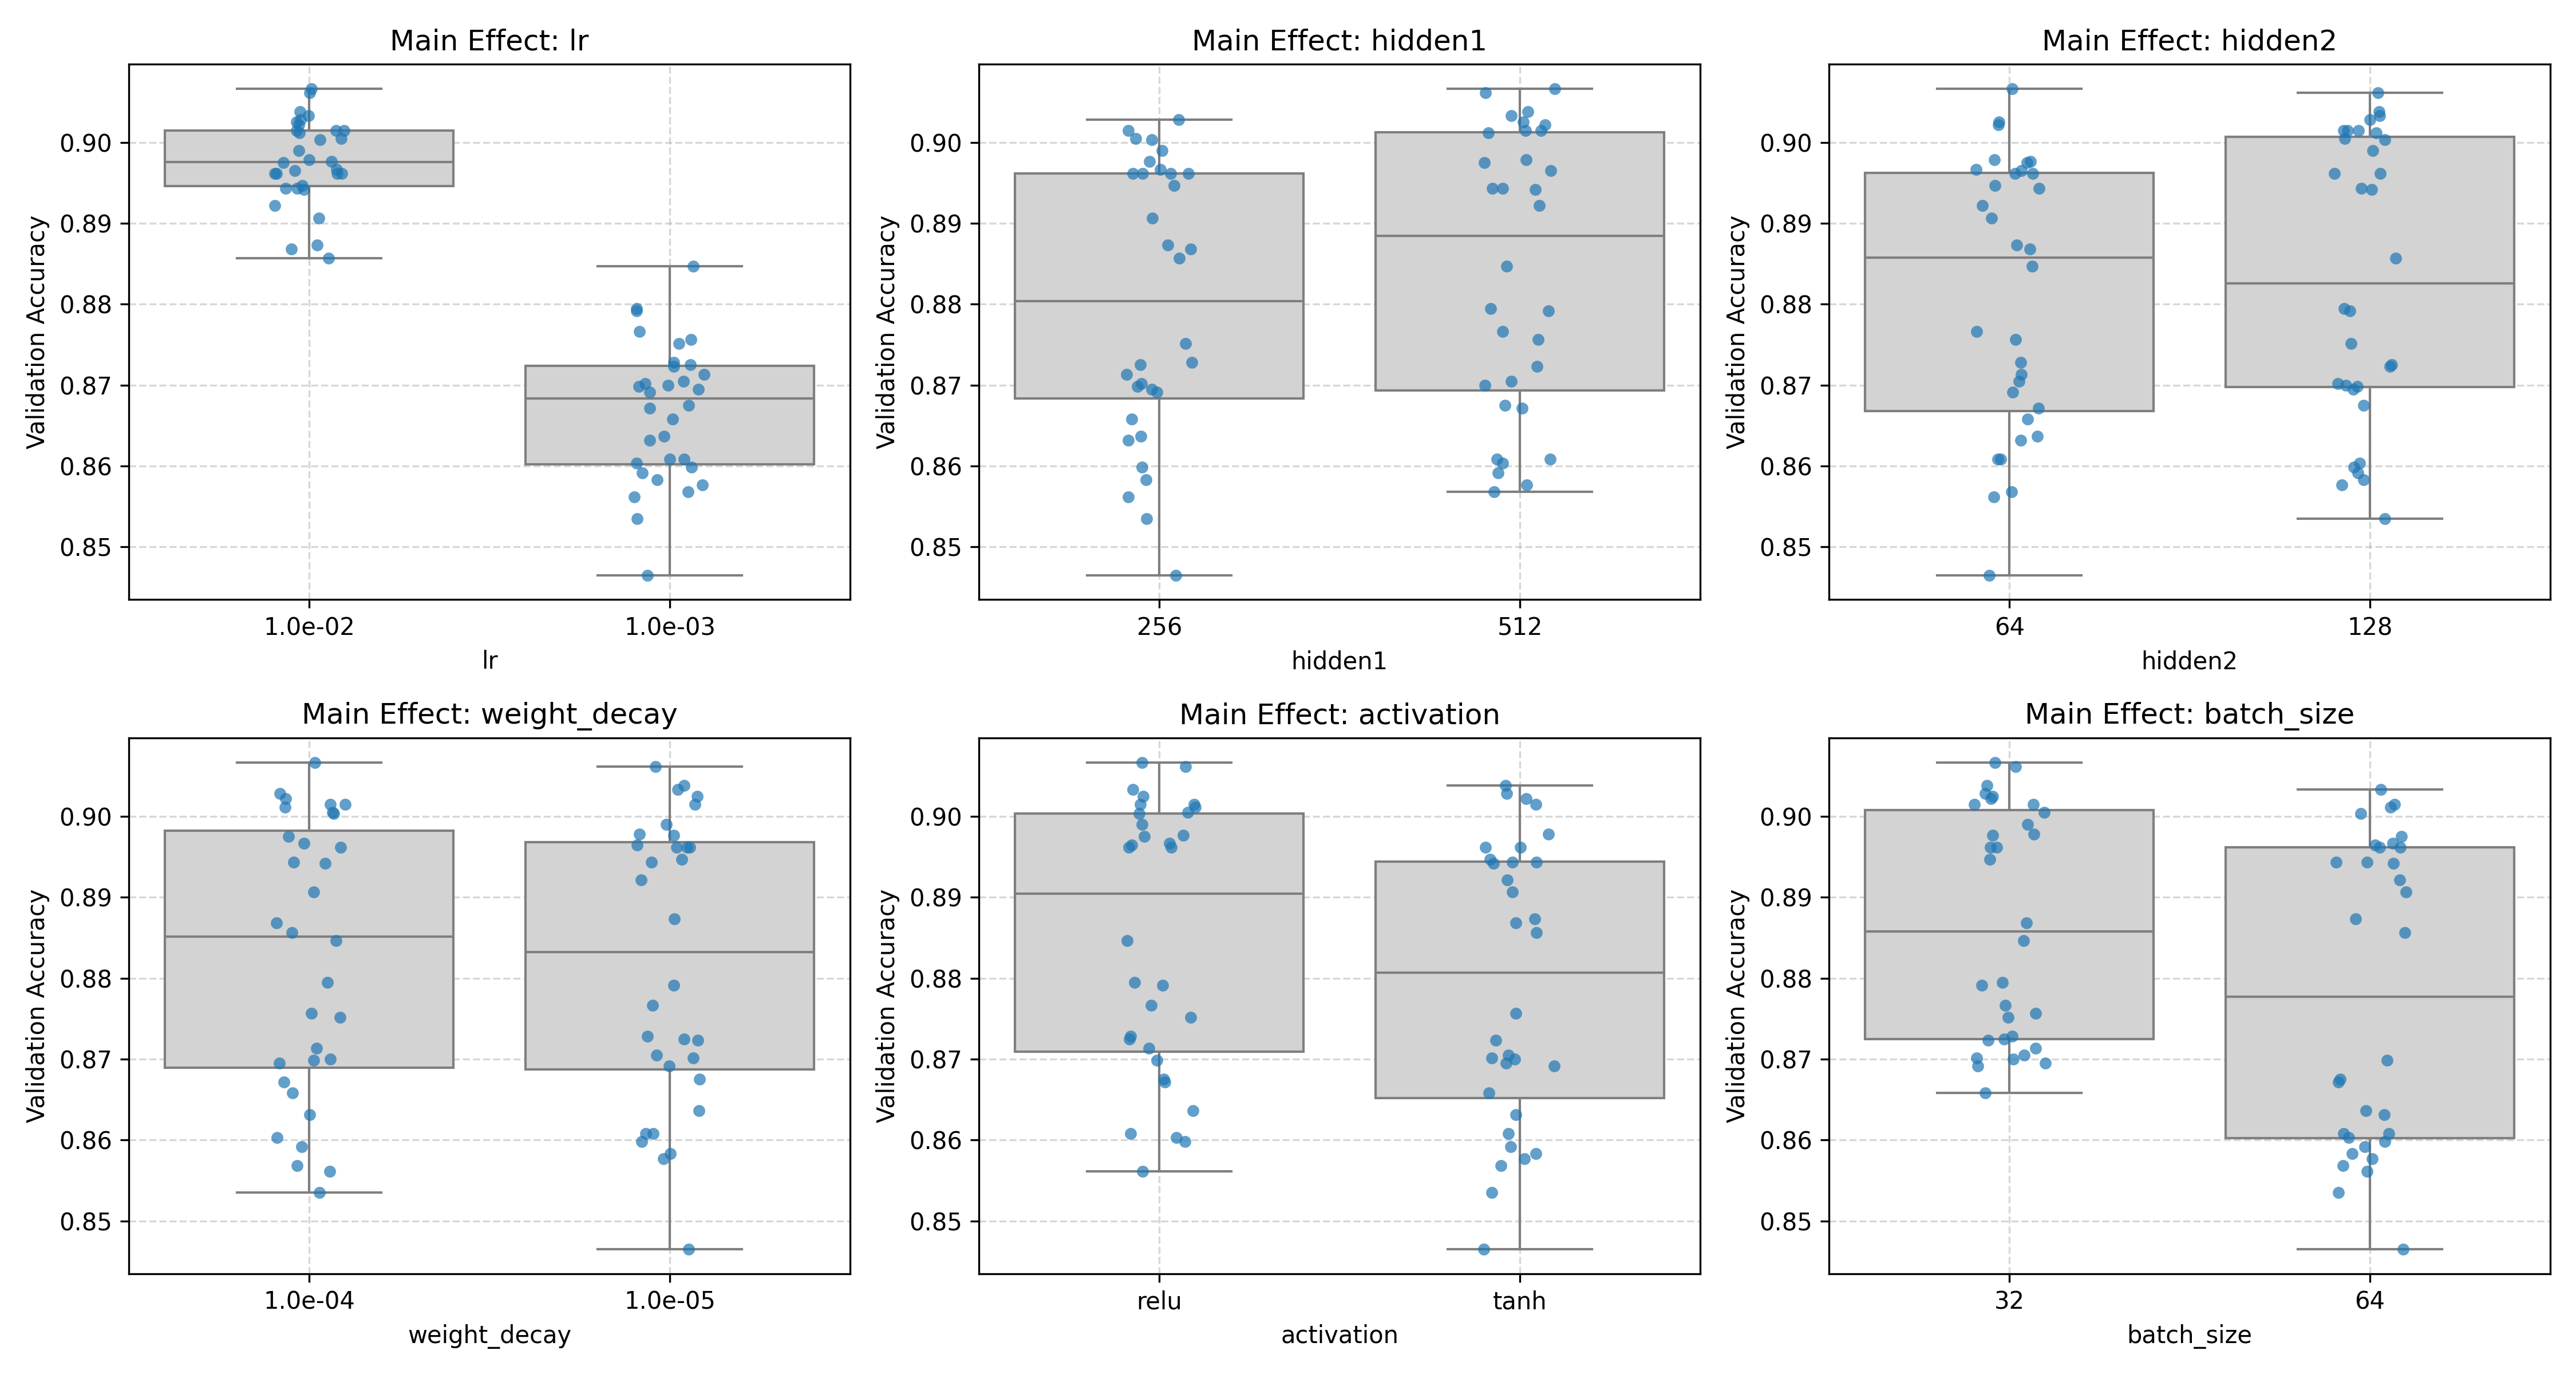
\includegraphics[width=0.8\linewidth]{../figures/search_1_marginal_effects.png}
    \caption{Marginal effects of hyperparameters (Stage I)}
    \label{fig:search1_marginal}
\end{figure}

The best configurations from this stage typically involve a larger first hidden layer ($512$), ReLU activation, a learning rate of $10^{-2}$, and a smaller batch size ($32$). The best validation accuracy achieved in this stage is approximately $0.9067$. However, noticeable overfitting is observed in subsequent full training runs. We will analyze this overfitting behavior in detail in the subsequent Experimental Results section, which directly motivated the introduction of dropout in Stage II.

\subsection{Stage II: Search with Dropout}

In the second stage, dropout is introduced to mitigate overfitting, and the search is refined around the previously identified promising configurations. The activation function and batch size are fixed (ReLU and $32$), while dropout probability is added as a key hyperparameter. In addition, other hyperparameters (learning rate, hidden dimensions, and weight decay) are re-searched to account for potential interactions with dropout.

Figure~\ref{fig:search2_corr} shows that dropout probability has the most significant impact on performance, with a strong negative correlation ($-0.81$), indicating that smaller dropout rates perform better. Among the tested values, $p=0.2$ achieves the best results. A mild positive correlation is again observed for the first hidden layer size.

\begin{figure}[H]
    \centering
    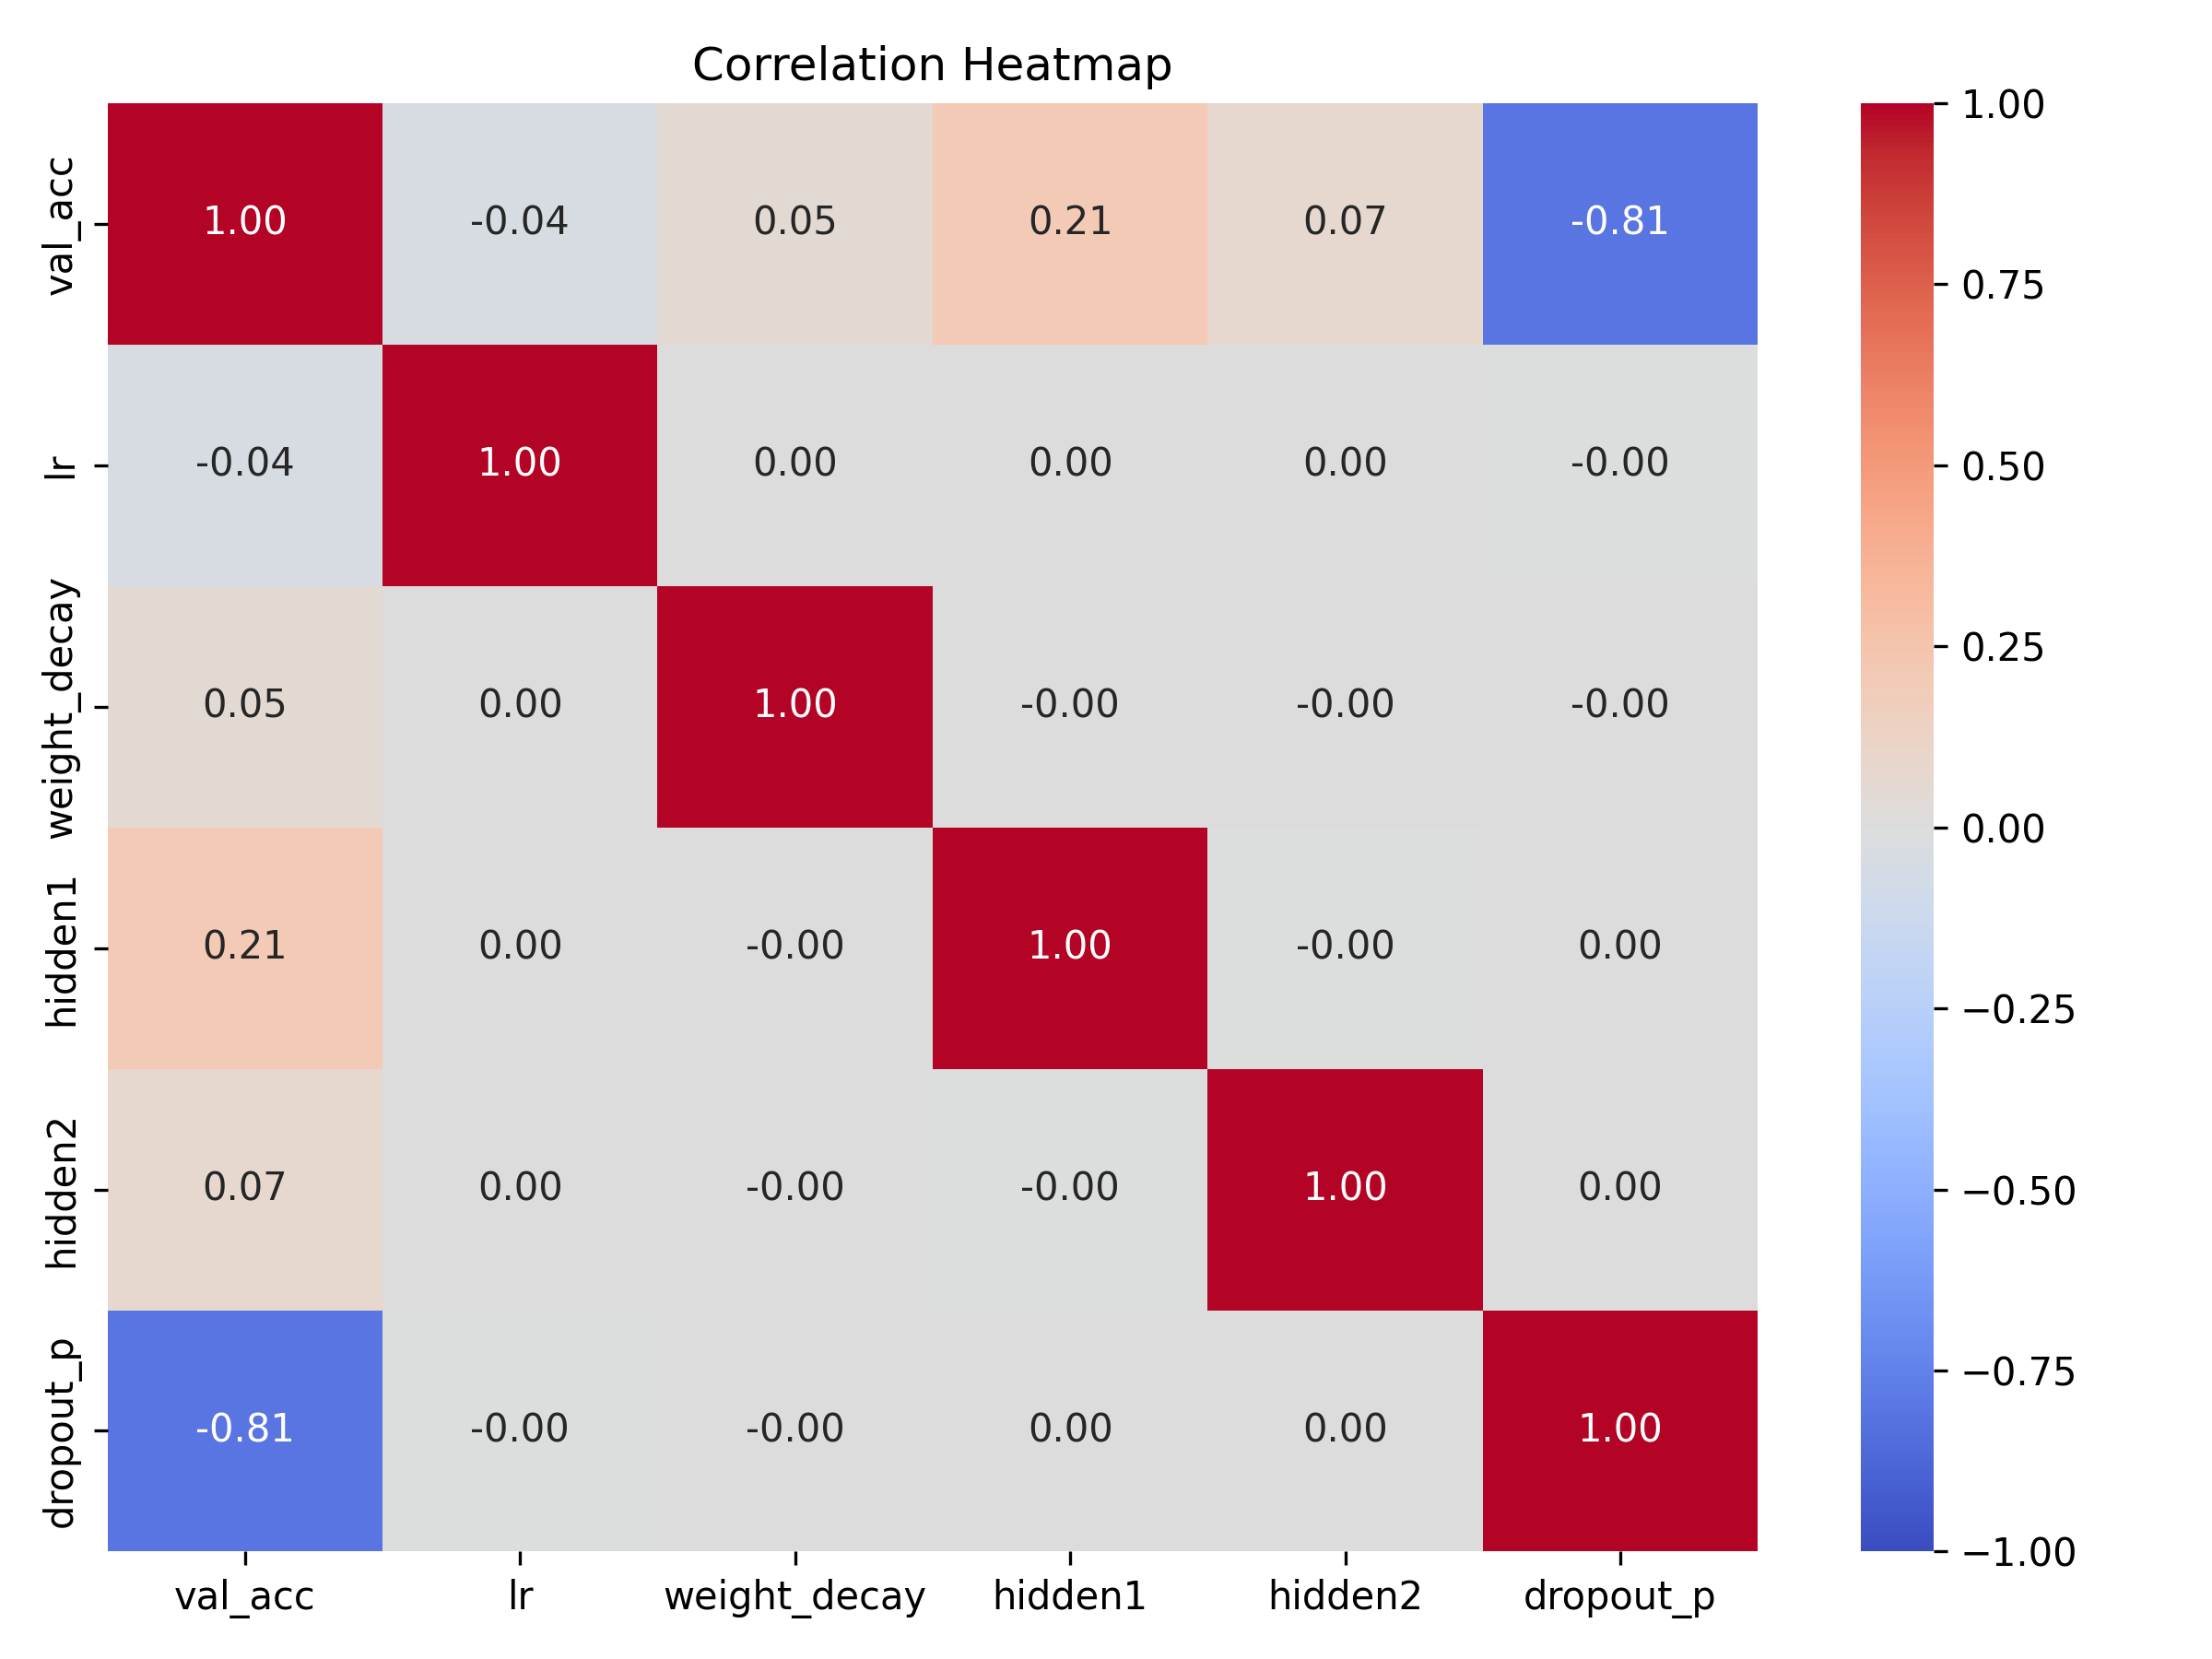
\includegraphics[width=0.7\linewidth]{../figures/search_2_correlation_heatmap.png}
    \caption{Correlation between hyperparameters and validation accuracy (Stage II)}
    \label{fig:search2_corr}
\end{figure}

This observation is further confirmed by the marginal effects shown in Figure~\ref{fig:search2_marginal}, where $p=0.2$ consistently outperforms larger dropout rates.

\begin{figure}[H]
    \centering
    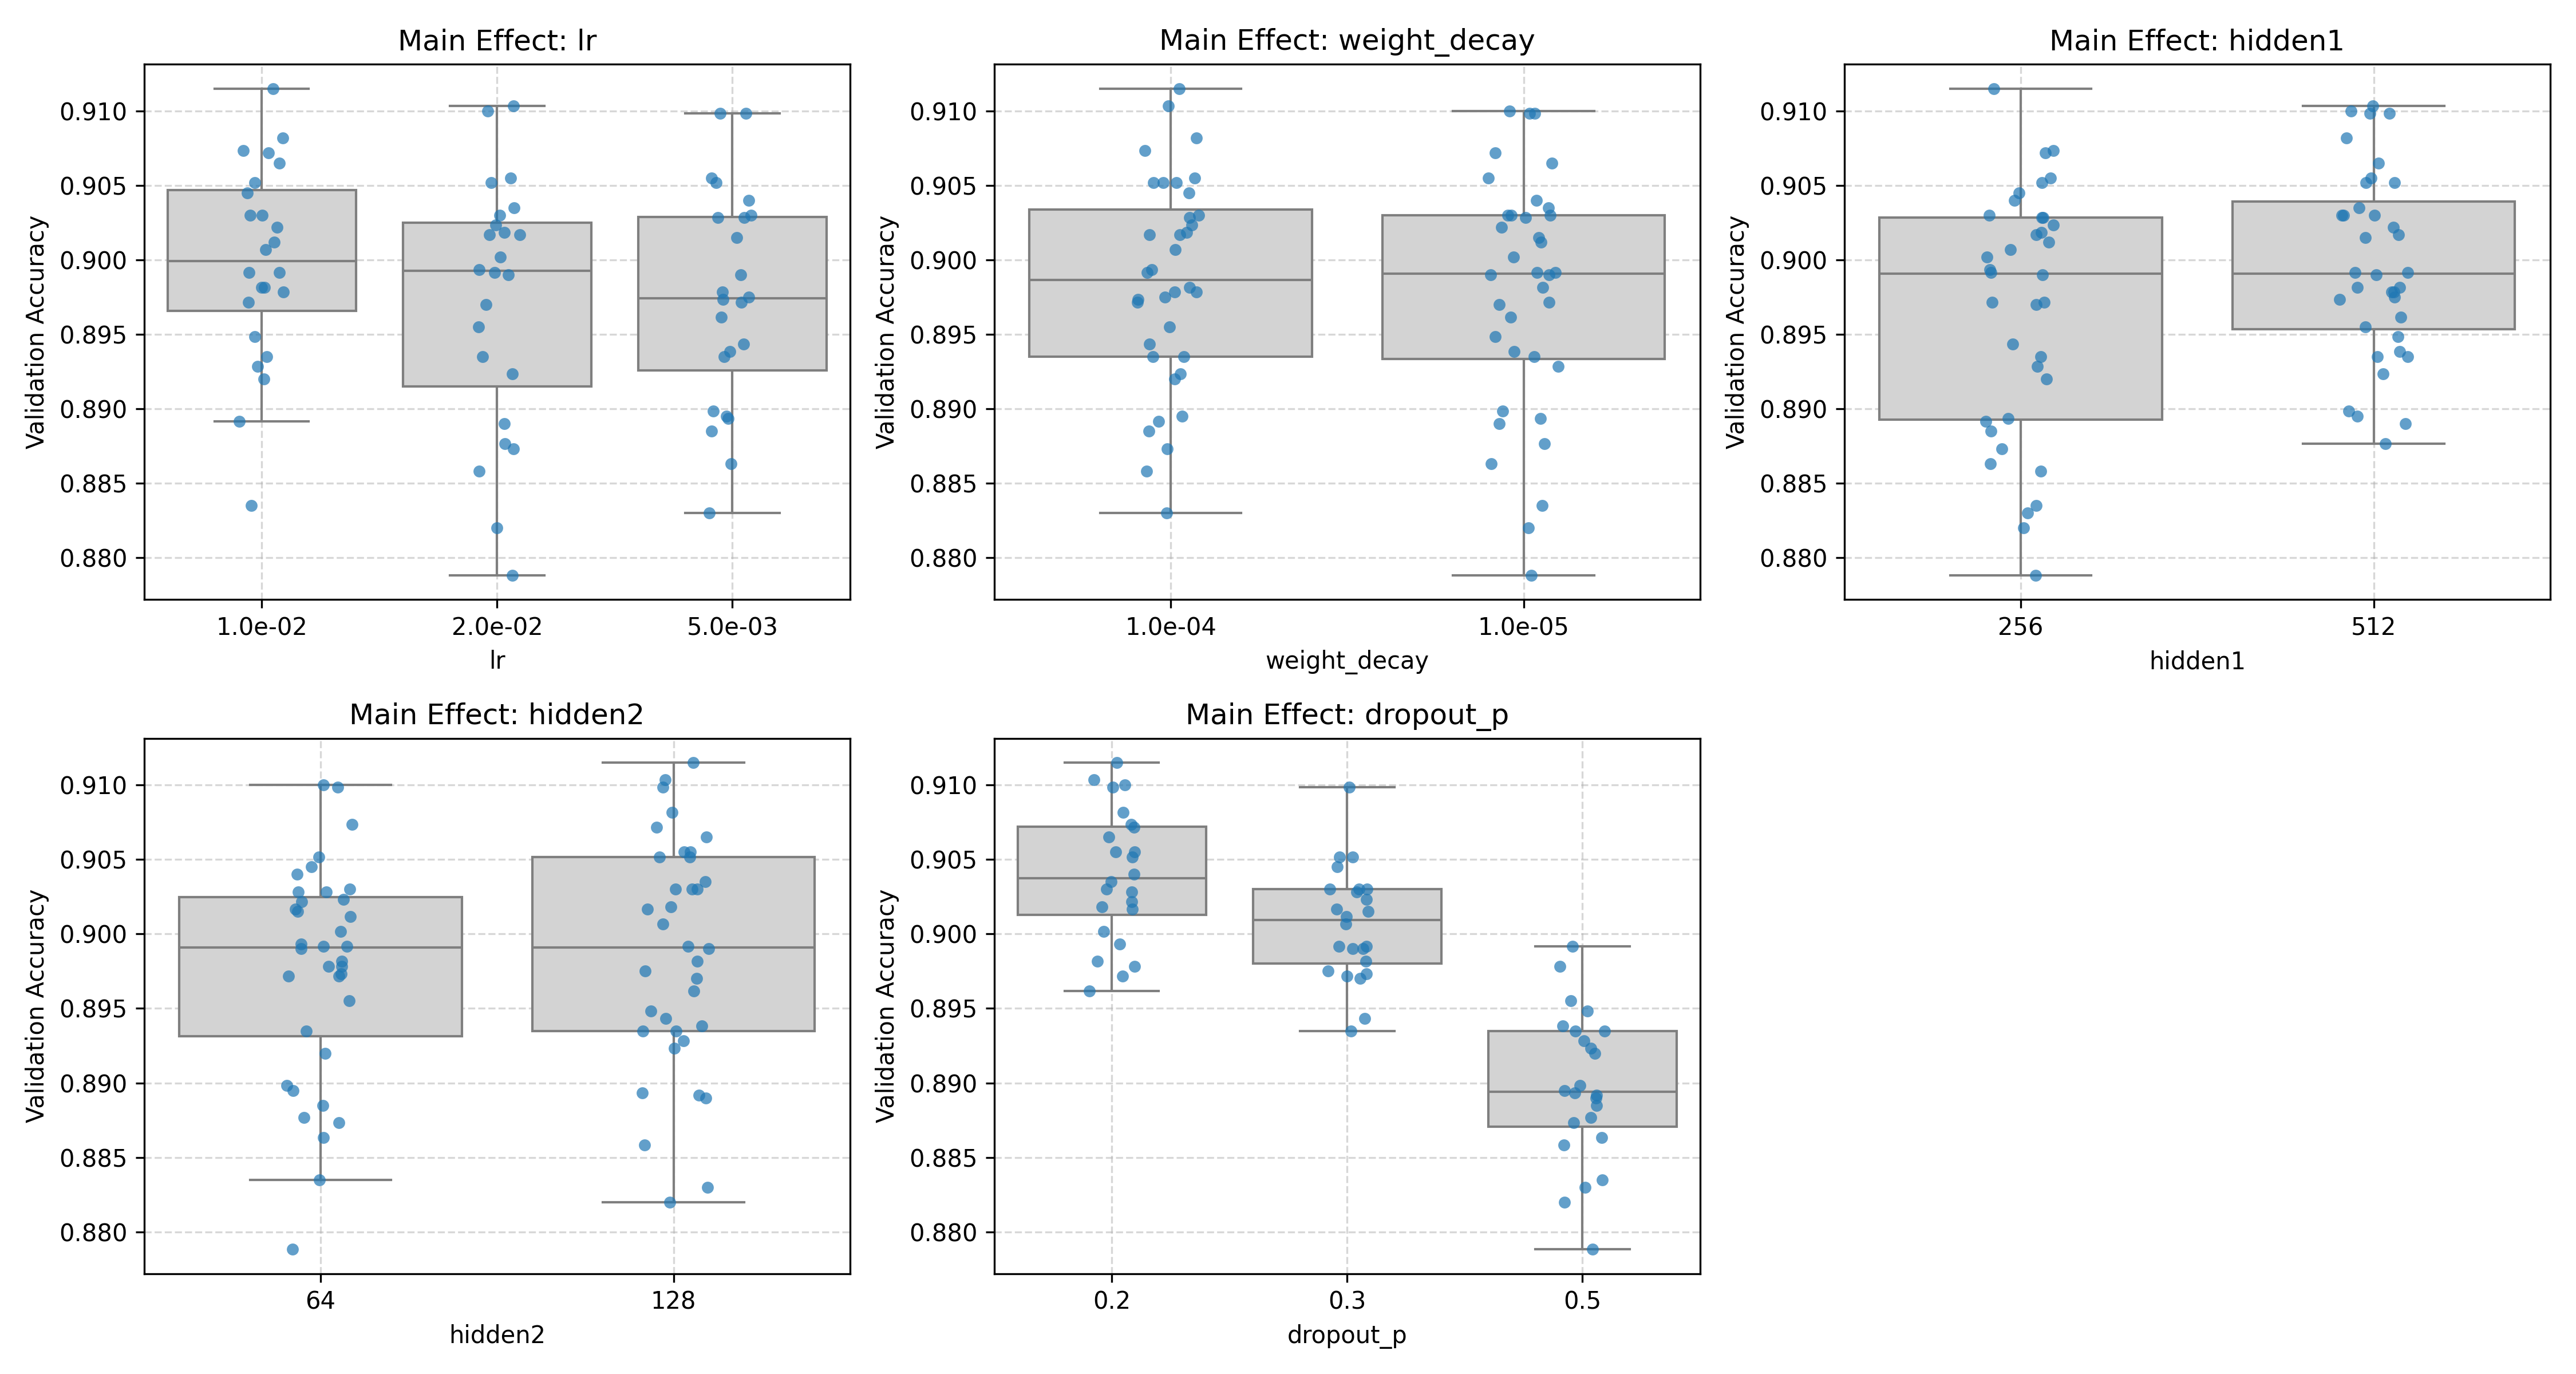
\includegraphics[width=0.8\linewidth]{../figures/search_2_marginal_effects.png}
    \caption{Marginal effects of hyperparameters (Stage II)}
    \label{fig:search2_marginal}
\end{figure}

The best configurations achieve validation accuracy above $91\%$, representing an improvement over the baseline without dropout.

\subsection{Final Hyperparameter Selection}

Based on the top-performing configurations identified in Stage II, several candidate settings are further evaluated under extended training (100 and 200 epochs), and their validation performance is summarized in Table~\ref{tab:final_hparams}.

\begin{table}[H]
\centering
\caption{Candidate hyperparameter configurations and validation performance}
\label{tab:final_hparams}
\begin{tabular}{c c c c c c c c c}
\toprule
Epochs & LR & WD & H1 & H2 & Dropout & Batch & Act & Val Acc \\
\midrule
200 & 0.01 & $1\mathrm{e}{-4}$ & 256 & 128  & 0.2 & 32 & ReLU & 0.9080 \\
100 & 0.01 & $1\mathrm{e}{-4}$ & 256 & 128  & 0.2 & 32 & ReLU & 0.9112 \\
200 & 0.02 & $1\mathrm{e}{-4}$ & 512 & 128 & 0.2 & 32 & ReLU & \textbf{0.9165} \\
100 & 0.02 & $1\mathrm{e}{-4}$ & 512 & 128 & 0.2 & 32 & ReLU & 0.9088 \\
\bottomrule
\end{tabular}
\end{table}

Among these candidates, the configuration with $\text{lr}=0.02$, $\text{weight decay}=10^{-4}$, hidden dimensions $(512, 128)$, and dropout $p=0.2$ achieves the highest validation accuracy (0.9165) when trained for 200 epochs. This configuration is selected as the final hyperparameter setting.

It is worth noting that increasing the number of epochs does not consistently improve performance, as evidenced by the comparison across configurations. This suggests that training duration should be considered jointly with other hyperparameters.

The selected configuration is used in the subsequent Experimental Results section, where its training dynamics and generalization performance are analyzed in detail and directly compared against the baseline configuration without dropout.

\subsection{Remarks on Analysis}

The correlation analysis presented above captures marginal relationships between individual hyperparameters and validation accuracy. Interaction effects between hyperparameters are not explicitly modeled in this analysis. 

To partially address this limitation, the second-stage search re-optimizes multiple hyperparameters jointly after introducing dropout, allowing the search process to adapt to potential interactions in a practical manner.

\section{Experimental Results}

\subsection{Training Dynamics}

\begin{figure}[H]
    \centering
    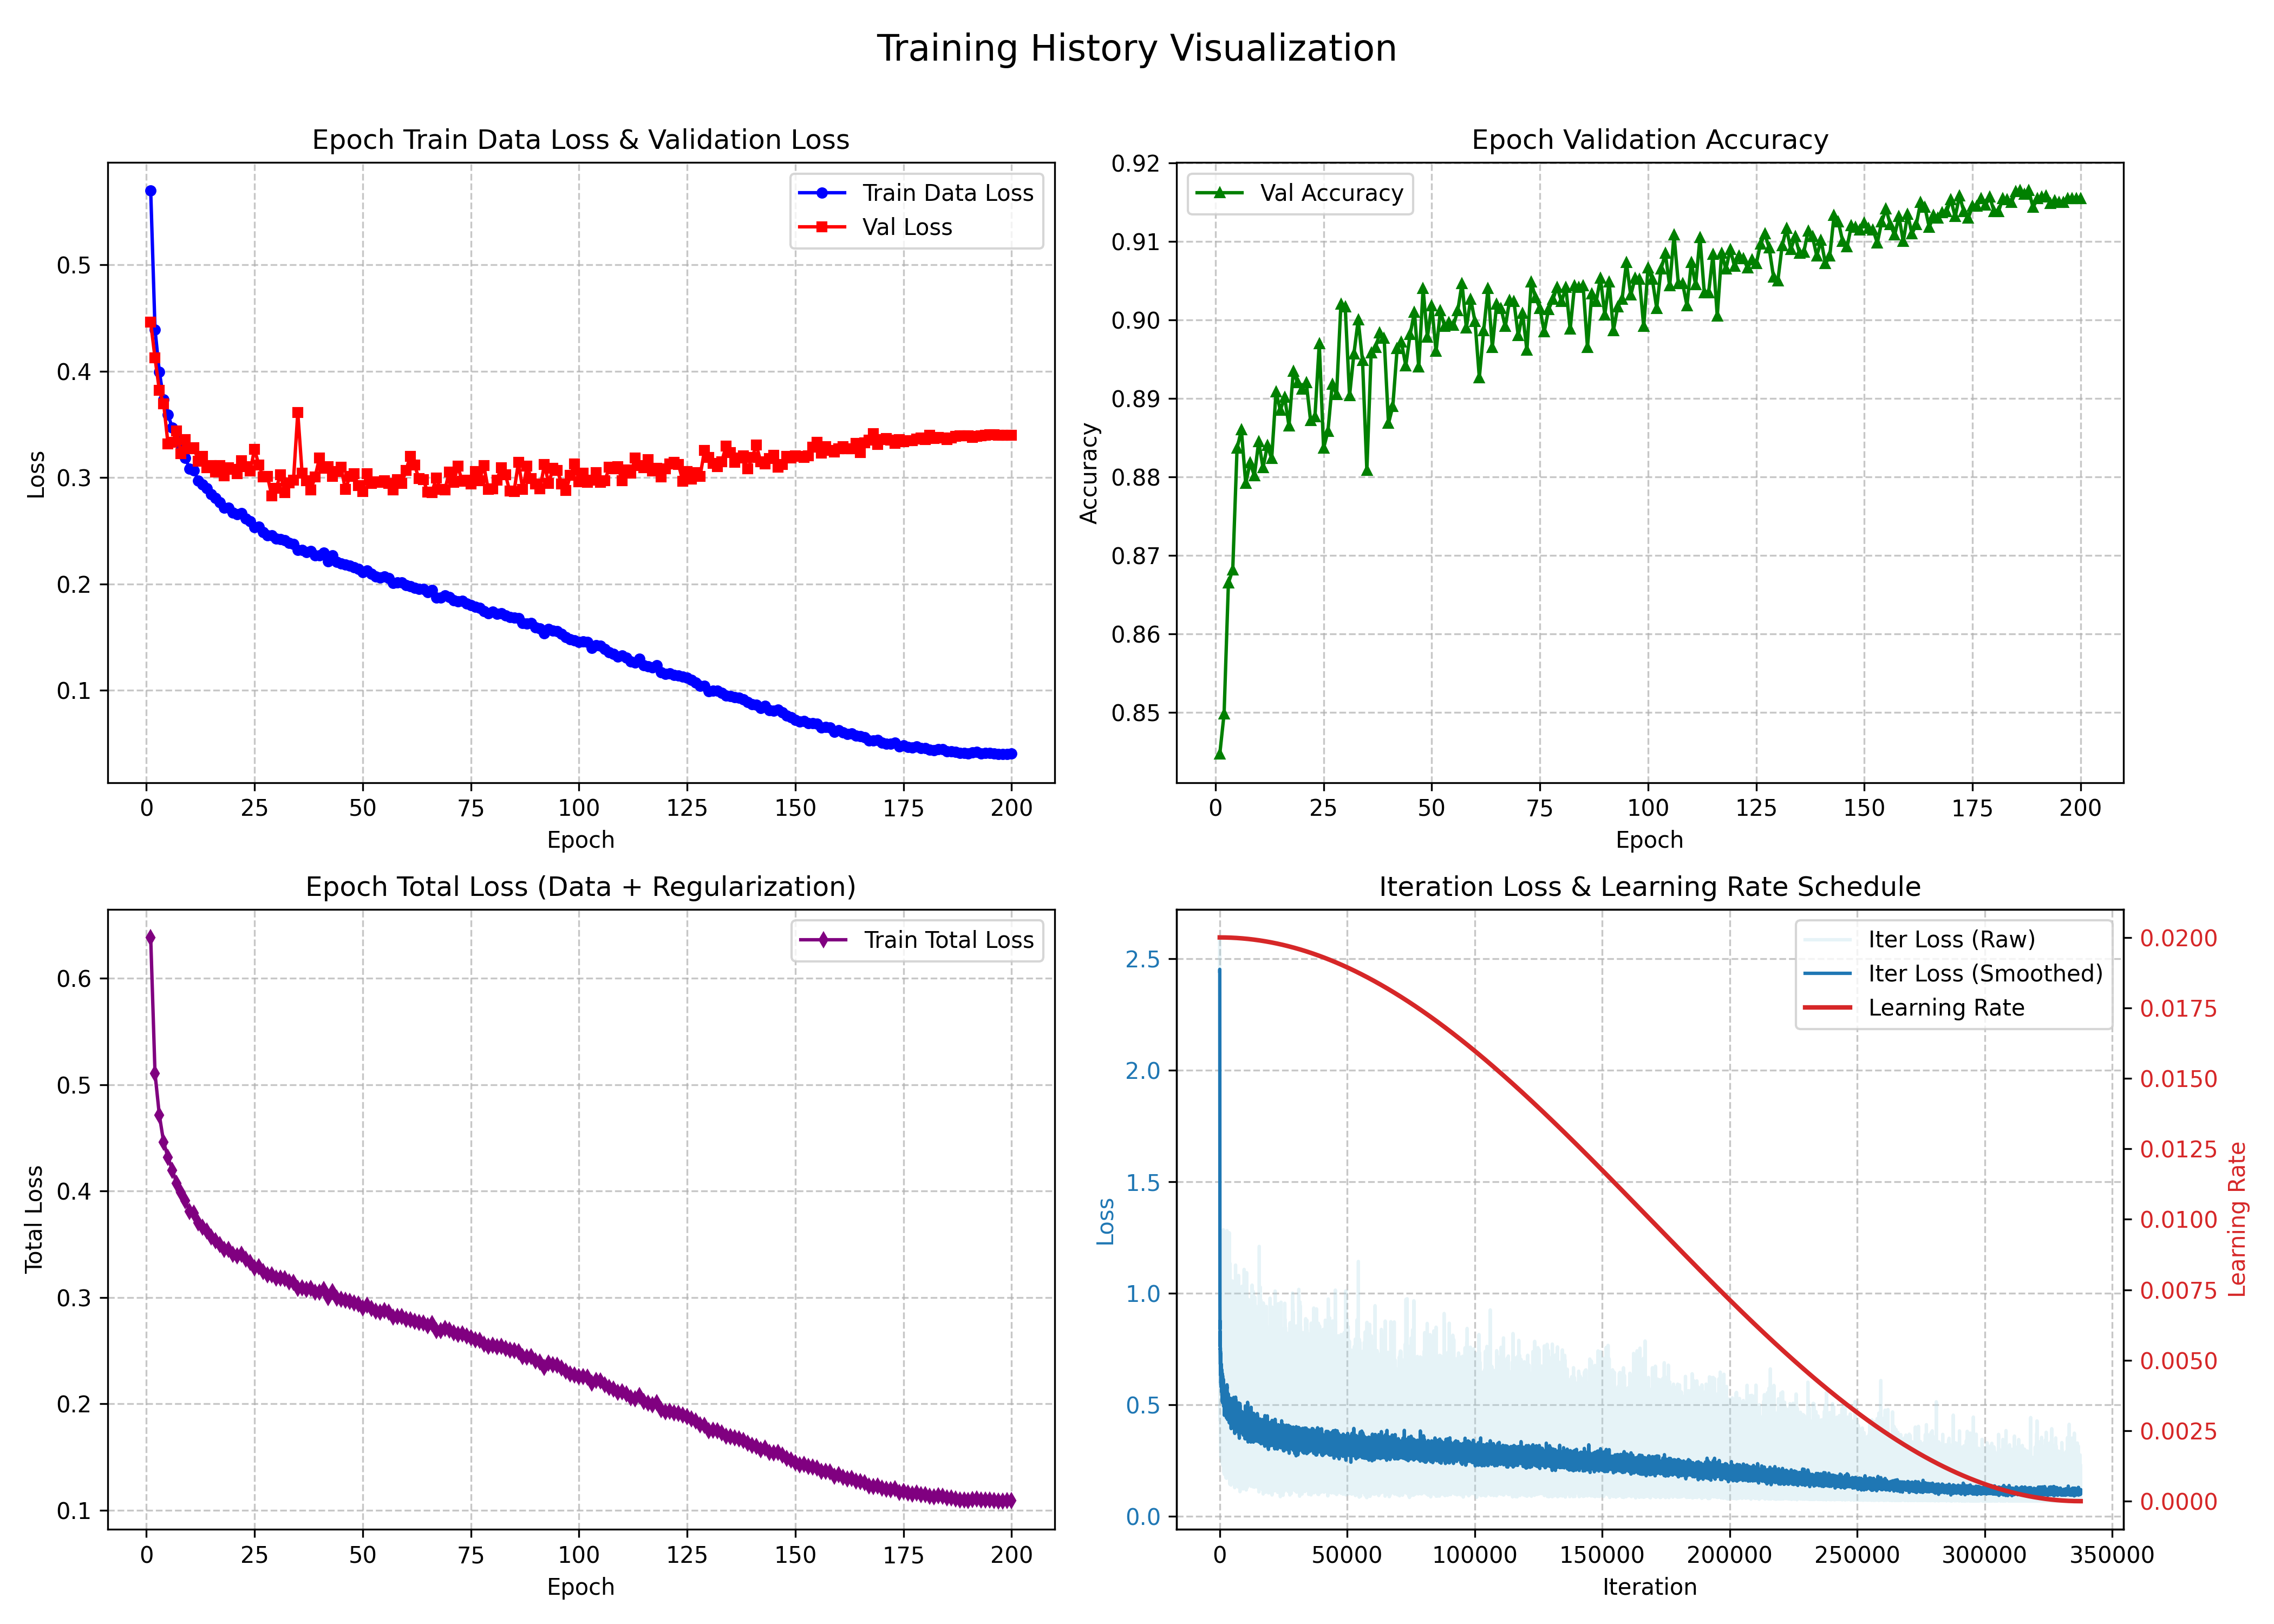
\includegraphics[width=0.9\linewidth]{../figures/history_plot.png}
    \caption{Training history under the selected hyperparameter configuration. Top-left: training data loss vs. validation loss. Top-right: validation accuracy. Bottom-left: total training loss (data + regularization). Bottom-right: iteration-level loss and learning rate schedule.}
    \label{fig:history_final}
\end{figure}

Figure~\ref{fig:history_final} presents the training dynamics of the final selected configuration. The training data loss decreases steadily throughout training, while the validation loss decreases in the early stage and then gradually stabilizes, followed by a mild increase. This indicates the onset of overfitting, with a significant gap emerging between the two curves as the training loss approaches zero while the validation loss plateaus around $0.33$.

The validation accuracy exhibits a different trend. It increases rapidly in the initial phase and continues to improve slowly even after the validation loss stops decreasing. The best model is obtained at a relatively late stage (around epoch 186), suggesting that validation accuracy and validation loss are not perfectly aligned during later training. This behavior likely occurs because the model's decision boundaries continue to refine—allowing it to correctly classify more samples and increase accuracy—but simultaneously, the model becomes increasingly overconfident in its remaining incorrect predictions. Since cross-entropy loss heavily penalizes highly confident errors, this overconfidence drives up the overall validation loss even as classification accuracy improves.

The bottom-right subplot shows the iteration-level training loss together with the cosine learning rate schedule. The learning rate decreases smoothly over time, which contributes to stable convergence in the later stage of training.

\begin{figure}[H]
    \centering
    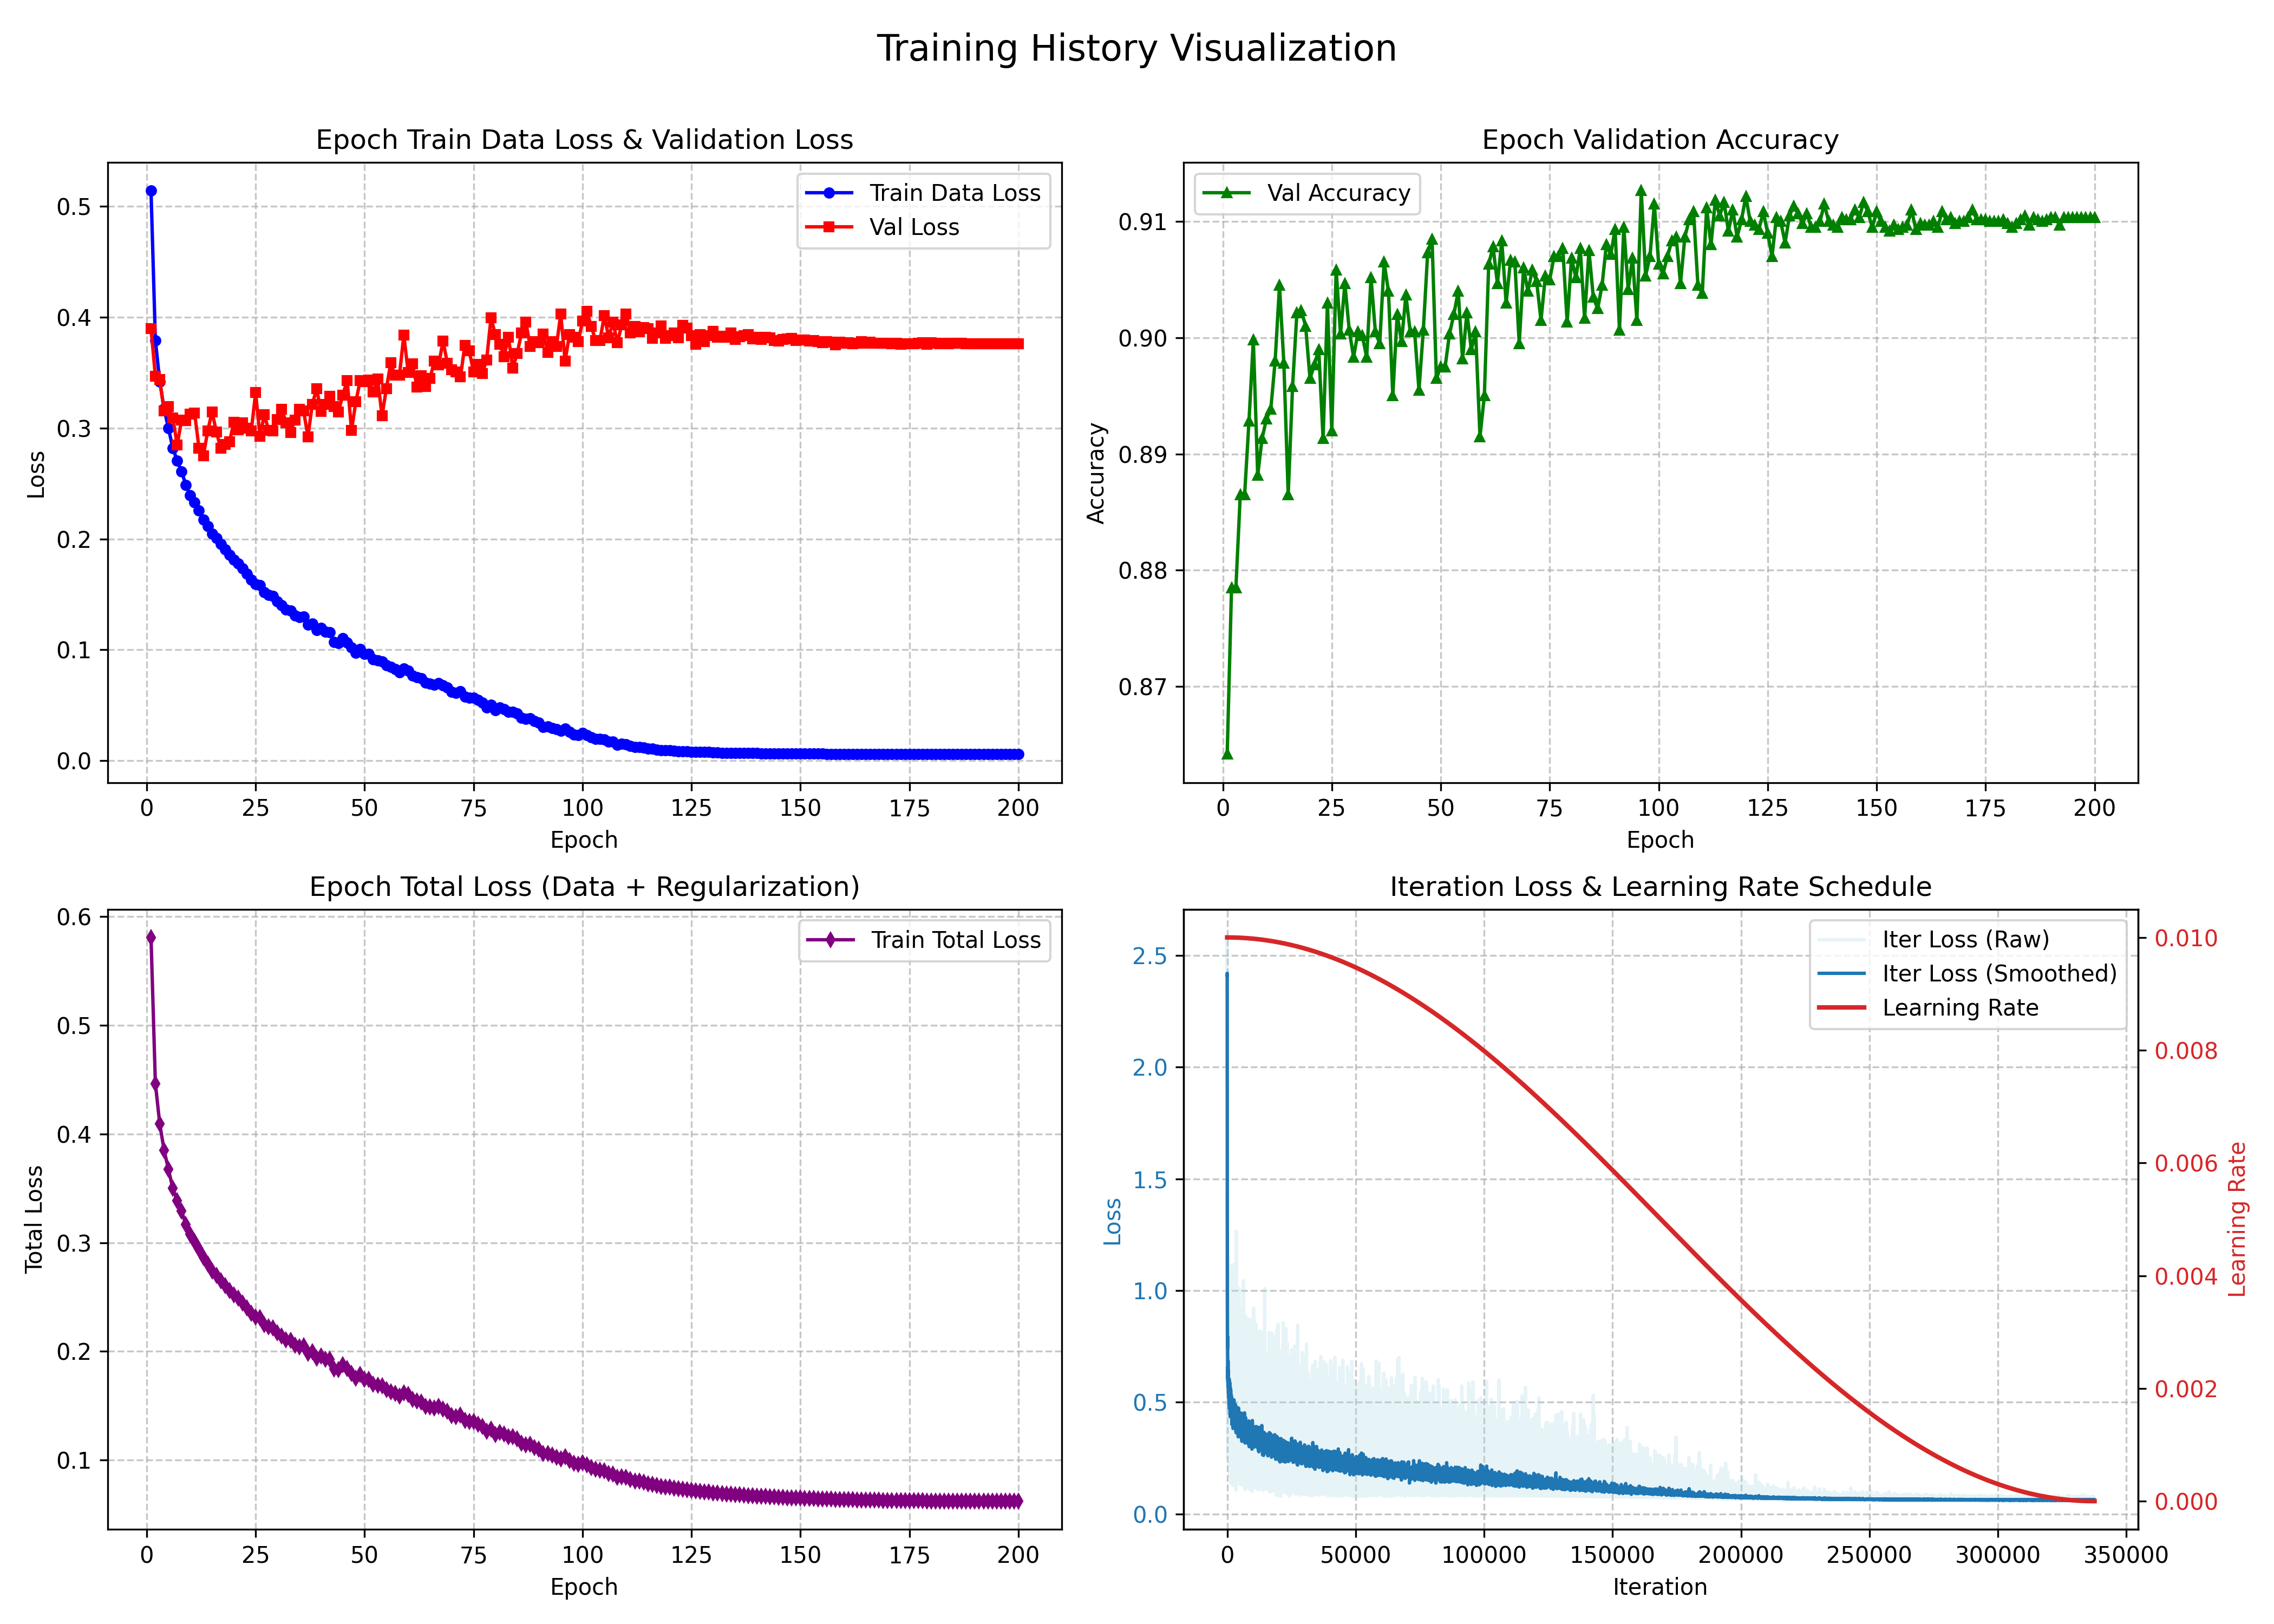
\includegraphics[width=0.9\linewidth]{../figures/overfit_history_plot.png}
    \caption{Training history without dropout (Stage I best configuration).}
    \label{fig:history_nodropout}
\end{figure}

To better understand the role of regularization, Figure~\ref{fig:history_nodropout} shows the training dynamics without dropout. In this case, the validation loss decreases only for approximately 15 epochs, after which it begins to oscillate and eventually increases, stabilizing at a higher level. In contrast, with dropout, the validation loss decreases for a longer period (around 30 epochs) and stabilizes at a lower value.

Moreover, without dropout, the validation accuracy quickly saturates and fluctuates around its peak, with the best model appearing relatively early (around epoch 96). With dropout, accuracy continues to improve gradually over a longer training horizon. This indicates that dropout effectively delays overfitting and allows the model to benefit from extended training.

It is also observed that optimization becomes slower when dropout is applied, as reflected by the more gradual decrease in training loss. This is expected due to the stochastic masking introduced during training, which increases gradient noise but improves generalization.


\subsection{Test Set Evaluation}

\subsubsection{Test Accuracy}
The final selected model achieves a test accuracy of $90.53\%$ on the held-out test set. This is slightly lower than the best validation accuracy ($0.9165$), which is expected since model selection is performed based on validation performance. The result indicates that the selected configuration generalizes reasonably well, with only a modest generalization gap.

\subsubsection{Confusion Matrix}
\begin{figure}[H]
    \centering
    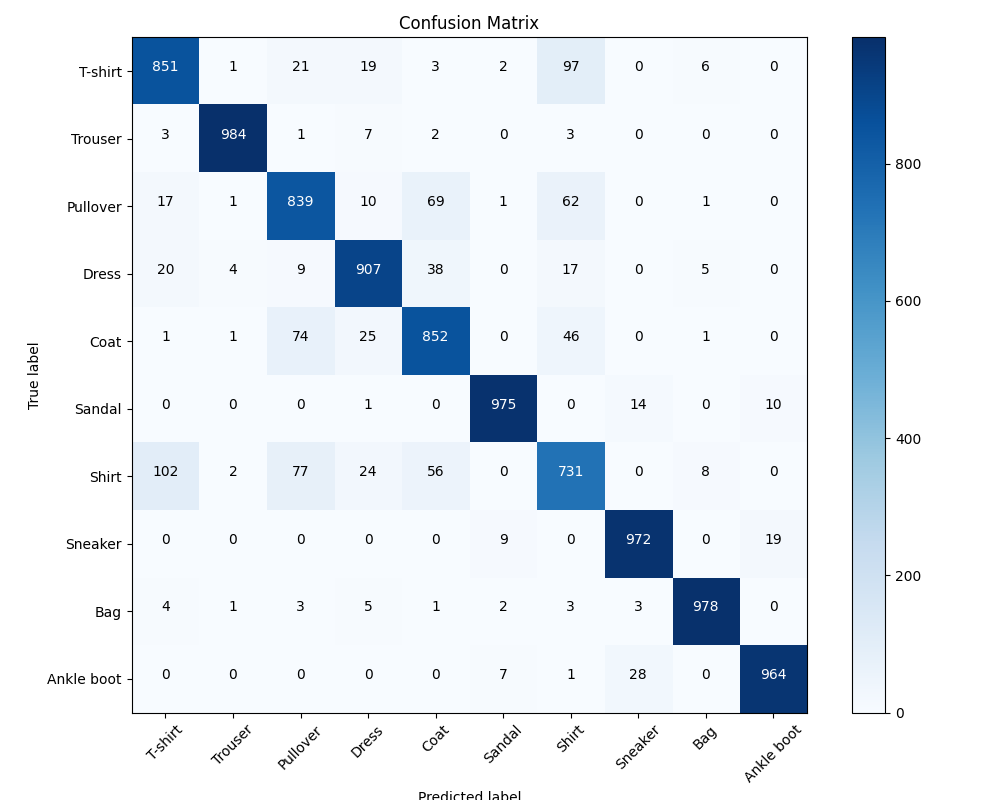
\includegraphics[width=0.7\linewidth]{../figures/cm_acc_90.5.png}
    \caption{Confusion Matrix on the test set}
\end{figure}

The confusion matrix shows that most errors occur between visually similar clothing categories. The most frequent misclassifications (with more than 40 instances) include:
\begin{itemize}
    \item Shirt $\leftrightarrow$ T-shirt
    \item Coat $\leftrightarrow$ Pullover
    \item Shirt $\leftrightarrow$ Pullover
    \item Shirt $\leftrightarrow$ Coat
\end{itemize}

These confusions reflect the similarity in shape and texture among upper-body garments. In contrast, footwear categories (e.g., \textit{Sandal}, \textit{Sneaker}, \textit{Ankle boot}) are relatively well separated overall, although occasional misclassifications still exist.

\subsubsection{Error Analysis}
\begin{figure}[H]
    \centering
    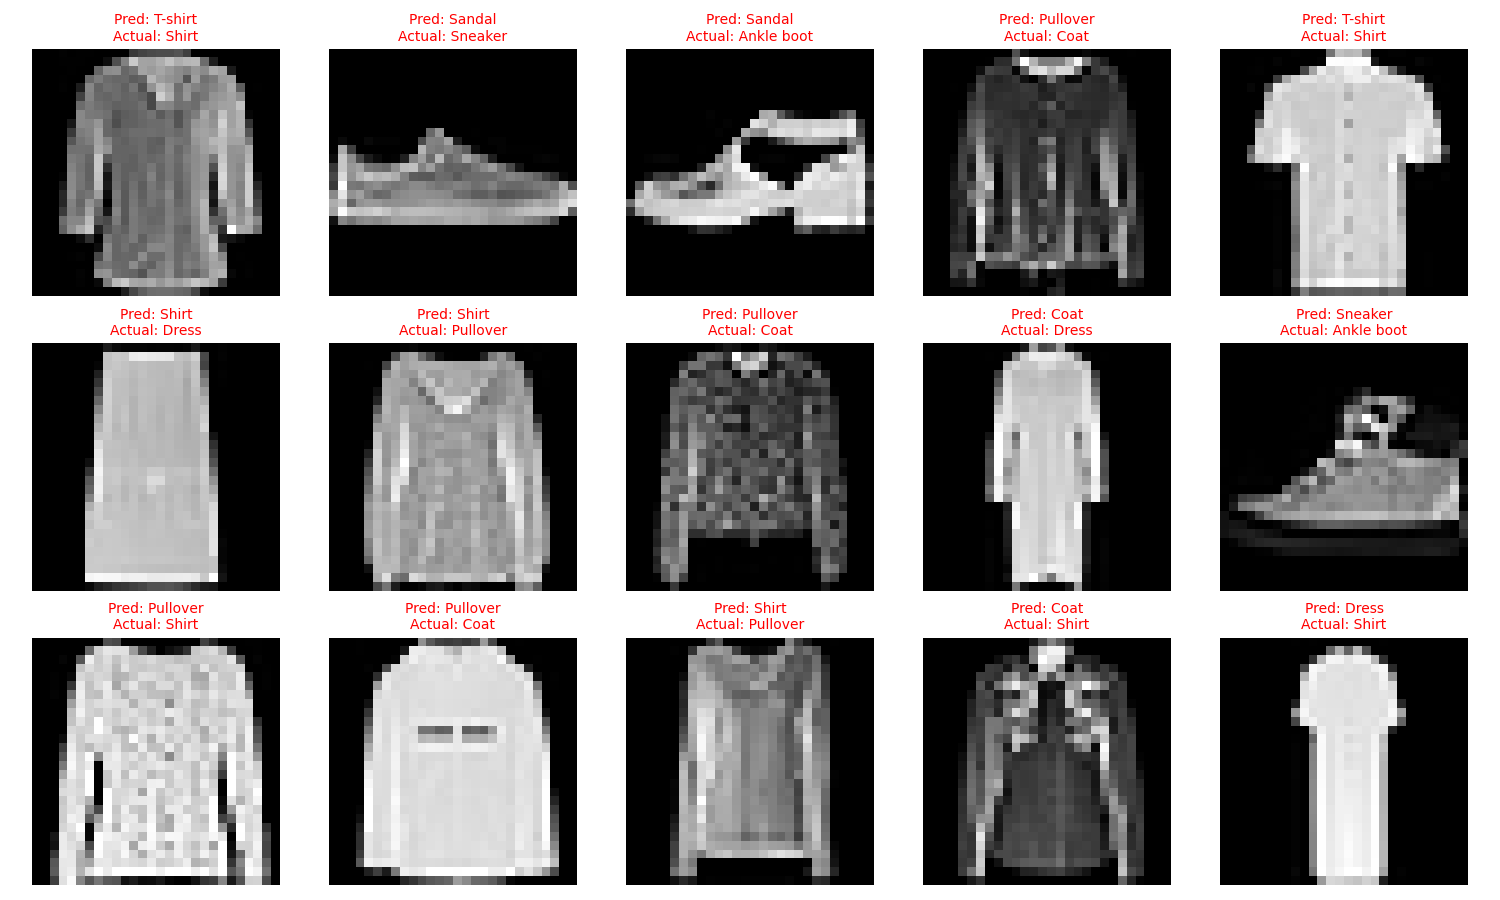
\includegraphics[width=0.8\linewidth]{../figures/error_analysis.png}
    \caption{Representative misclassified examples}
\end{figure}

Figure above shows representative misclassified samples. Several patterns can be observed:
\begin{itemize}
    \item \textbf{Clothing category ambiguity:} Many errors occur between similar garment types, such as \textit{Shirt} vs. \textit{T-shirt}, \textit{Pullover} vs. \textit{Coat}, and \textit{Dress} vs. \textit{Shirt}.
    \item \textbf{Ambiguous shapes:} Some samples lack clear structural features or contain atypical shapes, making them difficult to distinguish.
    \item \textbf{Footwear confusion:} Although footwear classes are generally well separated, occasional confusions (e.g., \textit{Sandal} vs. \textit{Sneaker}, \textit{Sneaker} vs. \textit{Ankle boot}) can still be observed. These cases are included here as representative examples rather than dominant error modes.
\end{itemize}

Overall, the errors are mainly driven by fine-grained visual similarity and ambiguous input patterns.

\subsection{Feature Representation Analysis}

\begin{figure}[H]
    \centering
    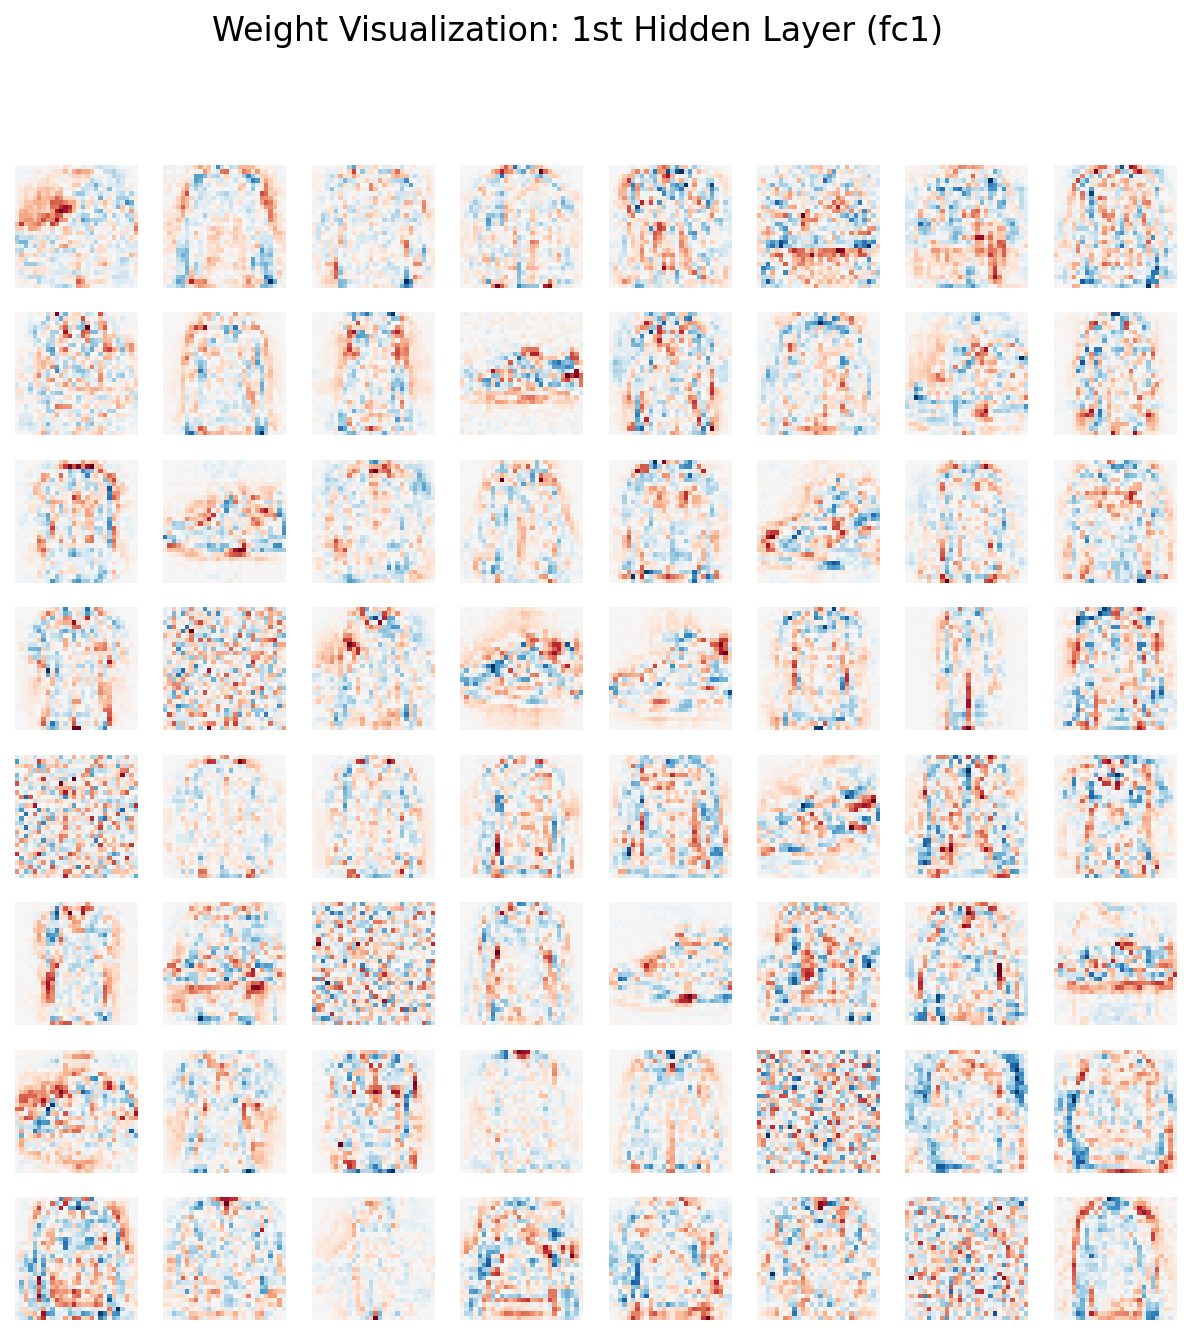
\includegraphics[width=0.8\linewidth]{../figures/fc1_weights_pattern.png}
    \caption{Visualization of first-layer weight vectors (64 neurons)}
\end{figure}

The first-layer weights are visualized as $28 \times 28$ patterns, revealing the types of features learned by the model. Many neurons capture meaningful spatial structures such as edges, contours, and localized regions.

To further illustrate this, several representative neurons are shown below.

\begin{figure}[H]
    \centering
    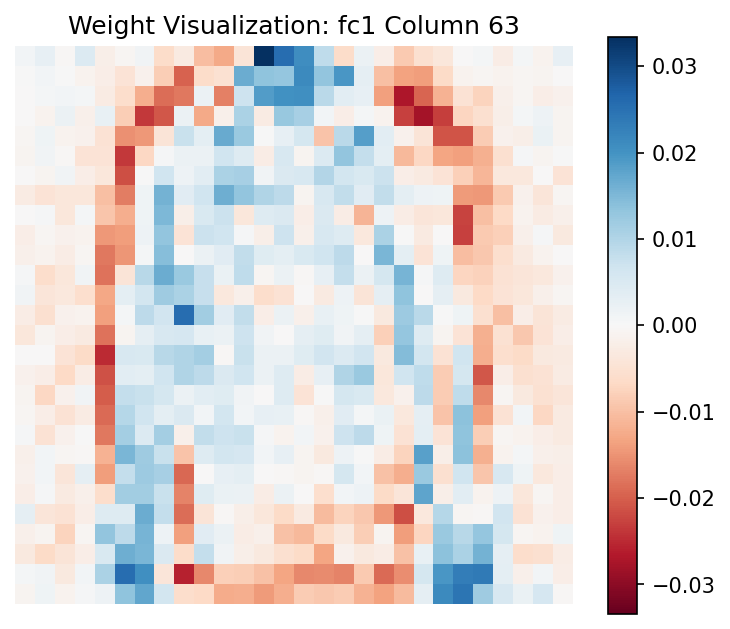
\includegraphics[width=0.22\linewidth]{../figures/fc1_weights_shirt.png}
    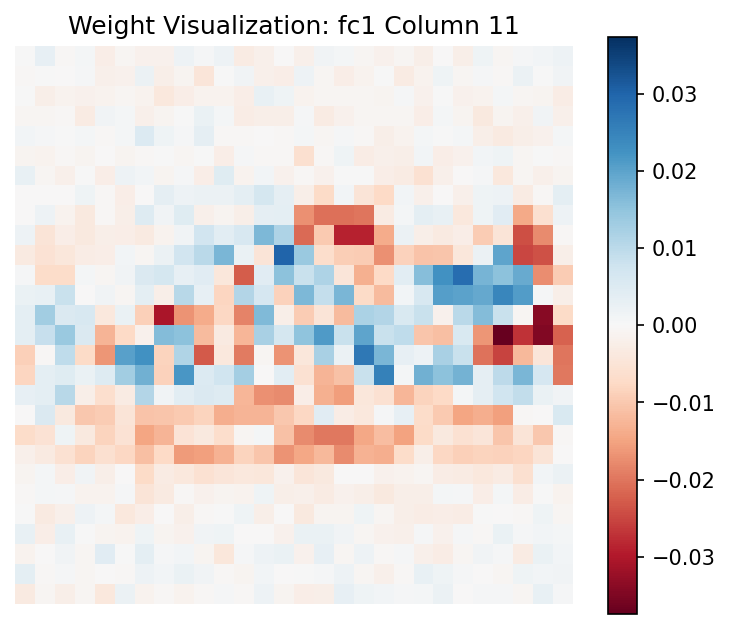
\includegraphics[width=0.22\linewidth]{../figures/fc1_weights_sneaker.png}
    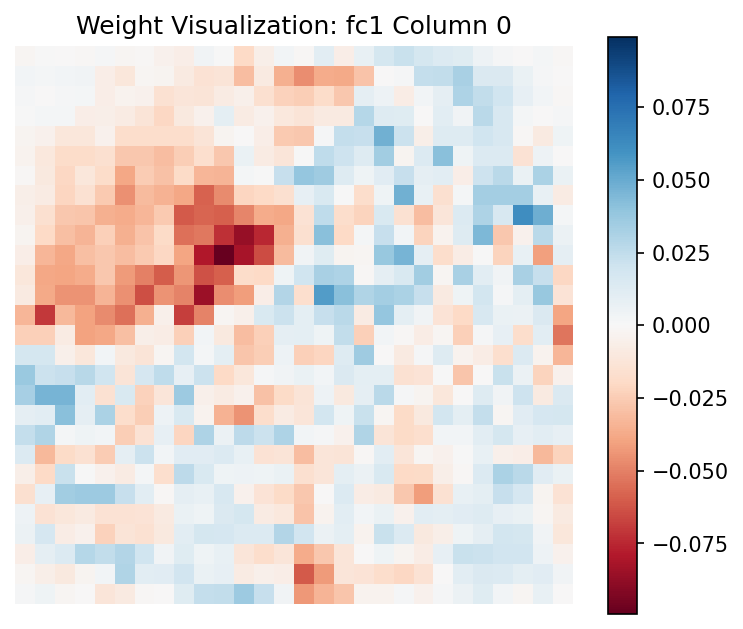
\includegraphics[width=0.22\linewidth]{../figures/fc1_weights_texture.png}
    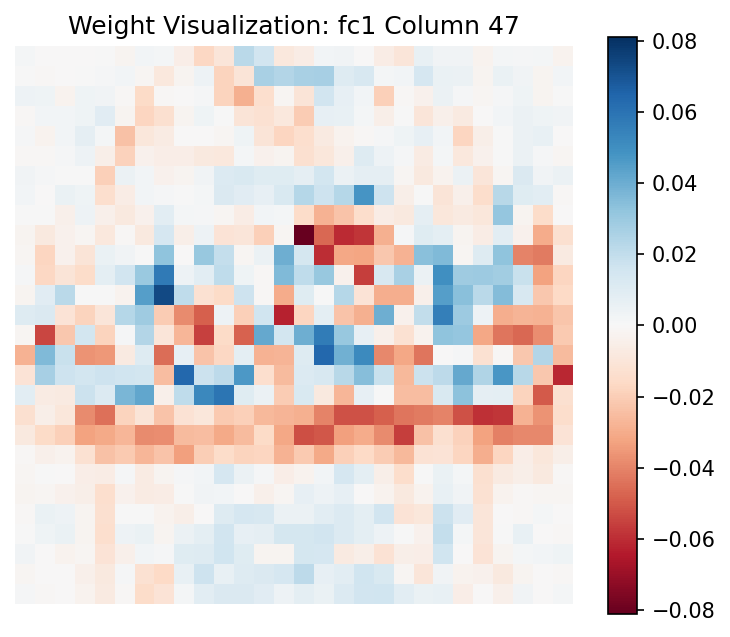
\includegraphics[width=0.22\linewidth]{../figures/fc1_weights_shoe&clothes.png}
    \caption{Examples of learned first-layer features}
\end{figure}

These visualizations suggest that:
\begin{itemize}
    \item Some neurons capture \textbf{clothing-related global shapes}, such as shirt-like outlines and upper-body structures.
    \item Some neurons respond to \textbf{footwear-related patterns}, capturing distinctive shoe shapes.
    \item Certain neurons encode \textbf{local textures or regions}, which may correspond to background or fabric patterns.
    \item A few neurons exhibit \textbf{mixed responses}, combining multiple semantic patterns (e.g., overlapping clothing and footwear features).
\end{itemize}

Overall, the learned representations demonstrate that even a simple MLP can extract semantically meaningful patterns from pixel inputs.

\section{Implementation Details}

\subsection{Project Structure}

The project is organized into several modular components:

\begin{itemize}
    \item \textbf{core/}: Contains fundamental building blocks, including activation functions (\texttt{ReLU}, \texttt{Sigmoid}, \texttt{Tanh}), layers (\texttt{Linear}, \texttt{Dropout}), loss function (\texttt{CrossEntropyLoss}), optimizer (SGD with momentum), learning rate schedulers (constant, step, linear, cosine), and a lightweight gradient control utility (\texttt{no\_grad}).
    
    \item \textbf{datasets/}: Provides data handling utilities. The \texttt{prepare\_data} function loads and splits the dataset, while \texttt{DataLoader} implements mini-batch iteration. A helper script is included for downloading Fashion-MNIST.
    
    \item \textbf{models/}: Implements the \texttt{ThreeLayerMLP} model, which composes linear layers, activation functions, and dropout into a unified architecture.
    
    \item \textbf{visualization/}: Contains scripts for analyzing results, including training history, confusion matrix, error cases, hyperparameter search, and learned weights.
    
    \item \textbf{tests/}: Includes basic unit tests for data processing and training logic, ensuring correctness of key components.
    
    \item \textbf{root directory}: Provides entry-point scripts, including \texttt{train.py} (training pipeline), \texttt{evaluate.py} (model evaluation), and \texttt{search.py} (hyperparameter search).
\end{itemize}

\subsection{Testing Strategy}

To ensure correctness, two complementary testing approaches are adopted:

\begin{itemize}
    \item \textbf{Component-level testing:} Core utilities such as data loading (\texttt{prepare\_data}, \texttt{DataLoader}) are verified through dedicated test scripts (e.g., \texttt{test\_dataset.py}) to ensure correct functionality.

    \item \textbf{Training pipeline sanity check:} The full training pipeline is validated by overfitting a small subset of the data (implemented in \texttt{test\_train.py}). Successful overfitting indicates that forward propagation, backward propagation, and parameter updates are working consistently.
\end{itemize}

\section{Conclusion}

This work demonstrates that a carefully implemented three-layer MLP can achieve strong performance on the Fashion-MNIST dataset, reaching a test accuracy of $90.53\%$. 

Through systematic hyperparameter tuning, it is shown that learning rate, batch size, activation function, hidden layer dimensions, and dropout all have noticeable impact on performance. In particular, dropout effectively mitigates overfitting and enables longer training, leading to improved generalization.

Analysis of training dynamics shows that validation accuracy may continue to improve even after validation loss stabilizes. This indicates that different evaluation metrics capture different aspects of model behavior.

Feature visualization further indicates that the model is able to learn meaningful spatial patterns from raw pixel inputs.

\section{Future Work}

Several directions can be explored to further improve this work:

\begin{itemize}
    \item \textbf{Model architecture:} Extend the current MLP to deeper networks or incorporate convolutional structures to better capture spatial information.
    
    \item \textbf{Regularization techniques:} Investigate additional methods such as batch normalization or data augmentation.
    
    \item \textbf{Optimization methods:} Explore adaptive optimizers (e.g., Adam) and more advanced learning rate schedules.
    
    \item \textbf{Hyperparameter search:} Apply more efficient search strategies such as Bayesian optimization to better explore high-dimensional spaces.
    
    \item \textbf{Evaluation:} Conduct more detailed analysis of robustness and generalization under distribution shifts.
\end{itemize}

\section*{Appendix}

\subsection*{Code Repository}
The complete source code is available at:
\href{https://github.com/Kevin-LD/fashion_mnist_mlp}{GitHub repository}

\subsection*{Model Weights}
The trained model weights can be downloaded from:
\href{https://drive.google.com/file/d/1oR0kwrEkUiJceKnIKqiBwuYCAAms9fPR/view?usp=sharing}{Google Drive link}

\end{document}
